\documentclass[11pt,a4paper]{article}
\usepackage[margin=25mm,headheight=14pt,headsep=8mm]{geometry}
\usepackage{fontspec}
\IfFontExistsTF{Liberation Serif}{%
  \setmainfont{Liberation Serif}%
}{%
  \setmainfont{Times New Roman}%
}
\IfFontExistsTF{Liberation Sans}{%
  \setsansfont{Liberation Sans}%
}{%
  \setsansfont[Path=../../../../../tools/books/.cache/fonts/,
    BoldFont=DejaVuSans-Bold.ttf,
    ItalicFont=DejaVuSans-Oblique.ttf,
    BoldItalicFont=DejaVuSans-BoldOblique.ttf]{DejaVuSans.ttf}%
}
\IfFontExistsTF{DejaVu Sans Mono}{%
  \setmonofont[Scale=0.86]{DejaVu Sans Mono}%
}{%
  \setmonofont[Path=../../../../../tools/books/.cache/fonts/,
    Scale=0.86,
    BoldFont=DejaVuSansMono-Bold.ttf,
    ItalicFont=DejaVuSansMono-Oblique.ttf,
    BoldItalicFont=DejaVuSansMono-BoldOblique.ttf]{DejaVuSansMono.ttf}%
}
\usepackage{amsmath,amssymb,amsthm}
\usepackage{microtype}
\usepackage{setspace}
\setstretch{1.15}
\usepackage{longtable,booktabs,array,calc}
\newcounter{none}
\usepackage{needspace}
\usepackage{graphicx}
\usepackage{fancyhdr}
\usepackage[authoryear,round]{natbib}
\usepackage{xcolor}
\definecolor{linkblue}{HTML}{004B87}
\PassOptionsToPackage{hyphens}{url}
\usepackage[unicode,colorlinks=true,allcolors=linkblue,bookmarksnumbered=true]{hyperref}
\usepackage{xurl}
\urlstyle{same}
\hypersetup{pdftitle={What Prediction Leaves Out: Relational Objecthood
and the Grounds of
Purpose},pdfauthor={},pdfsubject={Synthese Blinded Manuscript},pdfkeywords={Relational
objecthood; Predictive equivalence; Markov blankets; Organizational
closure; Biological individuality; Naturalized teleology}}
\setlength{\parindent}{1.15em}
\setlength{\parskip}{2pt}
\setlength{\emergencystretch}{2.5em}
\setcounter{secnumdepth}{2}
\widowpenalty=10000
\clubpenalty=10000
\providecommand{\tightlist}{\setlength{\itemsep}{2pt}\setlength{\parskip}{0pt}}
\providecommand{\passthrough}[1]{#1}
\pagestyle{fancy}
\fancyhf{}
\fancyhead[L]{\footnotesize What Prediction Leaves Out}
\fancyhead[R]{\footnotesize Synthese (Anonymized Submission)}
\fancyfoot[C]{\small\thepage}
\renewcommand{\headrulewidth}{0.25pt}
\fancypagestyle{plain}{\fancyhf{}\fancyfoot[C]{\small\thepage}\renewcommand{\headrulewidth}{0pt}}
\begin{document}
\thispagestyle{plain}
\begin{flushleft}
{\fontsize{17.5}{22}\selectfont\bfseries What Prediction Leaves Out:
Relational Objecthood and the Grounds of Purpose\par}
\vspace{8pt}
{\small\emph{Anonymized manuscript prepared for double-blind review at Synthese}\par}
\end{flushleft}
\vspace{6pt}
\hrule height 0.4pt
\vspace{8pt}
\noindent\textbf{Abstract}\quad Across computational mechanics,
predictive processing, active inference, and pattern-based metaphysics,
predictive compression and statistical boundaries are widely treated as
privileged guides to what persists as an individual and what its
activity is for. This article argues that observational and predictive
sufficiency systematically underdetermines both diachronic objecthood
and purposive explanation. Underlying our formal results is a
forward-marginalization asymmetry: predictive compression marginalizes
over past causal pathways to retain forward output distributions,
erasing the counterfactual invariance, restorative expenditure, and
genealogical contrasts required for individuation and teleology.
Governed by a typed principle of explanatory preservation, we defend a
three-criterion relational realism and a four-rung bearer-indexed
account of purpose within a self-contained stochastic regenerative
model. First, minimal predictive quotients vary non-monotonically with
protocol scope---yielding two, three, or four classes on the same four
initial configurations---and couple infinite-horizon birth streams while
erasing realized repair expenditure. Second, decoded symbolic
instructions fail to determine executable agency without physical gate
constraints, while partially observed viability separates finite-memory
from reactive control and resists fixed-sample zero-risk certification.
Third, proliferative investment can maximize expected lineage growth
while reducing individual survival. Fourth, scalar and dual-criterion
scores underdetermine functional norms, yet paid restoration and
full-policy growth attainment are jointly realizable.\par
\vspace{6pt}
\noindent\textbf{Keywords}\quad Relational objecthood; Predictive
equivalence; Markov blankets; Organizational closure; Biological
individuality; Naturalized teleology\par
\vspace{8pt}
\hrule height 0.4pt
\vspace{12pt}

\section{Introduction: the explanatory transfer
problem}\label{introduction-the-explanatory-transfer-problem}

Consider an engineered or biological device that suffers internal damage
to an active instruction register and restores that register by majority
vote from surviving internal copies before generating its next external
output. Compare it with an otherwise similar device whose active
register was never damaged. Suppose that, once restoration is complete,
the two devices induce exactly the same probability distribution over
all subsequent observable outputs. For the task of predicting future
output streams, recording whether initial damage occurred is strictly
redundant: an optimal predictive compression merges the undamaged and
restored histories into a single equivalence class. For reconstructing
whether \emph{this} individual bearer incurred a three-unit metabolic or
energetic repair expenditure, however, that erased distinction is
decisive. Now suppose further that switching from a conservative
maintenance mode to a proliferative mode increases the expected number
of descendants per cycle while lowering the probability that the
original individual survives intact. Describing the proliferative mode
as ``promoting the system's persistence'' or ``serving the organism's
adaptive optimum'' is systematically ambiguous. Its truth value depends
on whether the bearer of the explanation is the focal individual, an
enduring organizational form re-instantiated across tokens, or an
expanding lineage counted at a future census.

These cases exemplify a pervasive methodological hazard across
philosophy of science, cognitive science, and theoretical biology, which
we call the \emph{explanatory transfer problem}. Over the past three
decades, formidable formal frameworks have converged on predictive
sufficiency, data compression, and long-run statistical optimization as
foundational tools for individuating systems and explaining their
directedness. In metaphysics and philosophy of science, pattern realism
ties ontological commitment to non-redundant predictive compression
\citep{dennett1987, dennett1991, ladymanRoss2007, wimsatt2007}. In
complex systems and reinforcement learning, computational mechanics and
predictive state representations define minimal internal states as
equivalence classes of histories sharing conditional future
distributions
\citep{crutchfieldYoung1989, shaliziCrutchfield2001, littmanSuttonSingh2001, barnettCrutchfield2015}.
In cognitive neuroscience and theoretical biology, predictive processing
and the free-energy principle move even more ambitiously from
statistical conditional independence---formalized via Markov
blankets---to claims about autonomous individuality, self-organization,
and active goal-seeking
\citep{friston2010, friston2013, clark2013, parrPezzuloFriston2022}.
Meanwhile, inverse reinforcement learning and evolutionary optimization
routinely characterize purposeful behavior by fitting scalar value or
fitness functions under which observed trajectories emerge as optimal
\citep{puterman1994, ngRussell2000}.

Each of these formalisms achieves genuine success within its home
domain. Selective representation is indispensable to science: an output
predictor is not defective because it omits internal energetic
accounting, and a demographic branching model is not defective because
it aggregates retained parents with newborn offspring. Trouble begins
when success in a predictive or aggregative task is illicitly
transferred to underwrite a conclusion about causal realization,
diachronic persistence, executable agency, or functional purpose whose
truth conditions depend on distinctions that the predictive
representation has quotiented away. Recent critiques of Markov-blanket
metaphysics \citep{raja2021, bruineberg2022} and organizational
normativity \citep{corti2023, bich2024, cuciniello2026} have exposed
fragments of this gap from different angles, either questioning whether
statistical boundaries demarcate physical agents or asking whether
causal self-maintenance suffices for teleological norms. Yet what
remains missing is a unified formal and philosophical diagnosis of
\emph{exact} information loss across predictive, interventional,
genealogical, and evaluative descriptions---paired with constructive
conditions showing when these descriptions genuinely cohere in one and
the same process.

This article supplies that diagnosis and constructive synthesis.
Underlying our formal results is a structural
\emph{forward-marginalization asymmetry}: predictive sufficiency
marginalizes over past causal pathways and internal mechanisms to retain
only equivalence classes of forward observable distributions, whereas
diachronic objecthood and purposive explanation depend on counterfactual
perturbation stability, paid restorative work, and bearer-specific
selective or regulatory contrasts---precisely the modal, energetic, and
genealogical distinctions that forward marginalization erases.
Consequently, object individuation and purposive attribution must be
governed by a typed \emph{principle of explanatory preservation}: a
representation adequate for predicting a declared family of observables
licenses an inference about persistence, causal mechanism, or purpose
only if---together with explicitly stated auxiliary premises---it
preserves the invariants required by that target claim at its stated
grain of precision. Neither predictive equivalence nor behavioral
optimality delivers ontology or teleology for free. Instead:

\begin{enumerate}
\def\labelenumi{\arabic{enumi}.}
\tightlist
\item
  \textbf{Constrained relational objecthood.} Against both substance
  essentialism and pure predictive instrumentalism, an organized process
  warrants defeasible realist commitment as an enduring individual to
  the extent that its internal relations jointly satisfy three
  exclusionary criteria: \emph{(i) non-trivial predictive--control
  compression} across declared observation protocols, \emph{(ii)
  counterfactual invariance under targeted structural and environmental
  interventions} \citep{hacking1983, woodward2003, craver2007}, and
  \emph{(iii) realization-cost and constraint accountability}, whereby
  at least one enabling boundary or operational constraint is
  endogenously maintained rather than passively inherited or externally
  imposed \citep{jonas1966, rosen1991, montevilMossio2015}.
\item
  \textbf{Bearer-indexed grounds of purpose.} Against both
  scalar-optimization imperialism and eliminativist skepticism,
  purposive explanation is neither a relabeling of stationary
  distributions nor a monolithic biological primitive. Every well-formed
  functional or purposive claim is indexed to a
  quadruple---\emph{diachronic bearer, contrast class, causal
  realization, and evaluative ground}---stratified across four
  non-interchangeable levels: \emph{(Rung 1) systemic causal
  contribution} \citep{cummins1975}, \emph{(Rung 2) endogenous
  regulatory and organizational viability}
  \citep{rosenblueth1943, mossio2009, diPaolo2005, bich2024},
  \emph{(Rung 3) historical stabilization via differential retention or
  differential reproduction}
  \citep{wright1973, millikan1984, godfreySmith1994, garson2019}, and
  \emph{(Rung 4) reflective practical and moral normativity}
  \citep{korsgaard1996, scanlon1998, street2006}.
\item
  \textbf{Constructive joint realizability.} Warnings against conflation
  would be methodologically sterile if repair, resource accounting,
  internal execution, and long-run demographic performance could only
  ever be exhibited in disconnected toy models. By constructing a
  self-contained stochastic regenerative model \(\mathcal{M}\) and
  proving all formal claims directly (with complete derivations in the
  Appendix), we show both \emph{where} predictive and evaluative
  reductions provably fail and \emph{exactly when} paid physical
  restoration, gate-mediated internal execution, genealogical
  continuity, and optimal expected lineage growth are jointly realized
  by a single damaged founder and its descendants.
\end{enumerate}

The paper proceeds in six steps. Section 2 formalizes protocol-indexed
predictive equivalence, establishes the typed preservation and
belief-quotient conditions, and defends our three-criterion account of
relational objecthood against pure compressionism and Markov-blanket
metaphysics. Section 3 introduces the unified stochastic regenerative
model \(\mathcal{M}\), proving the two--three--four task-partition
separation, repair-cost erasure, and the von Neumann separation between
decoded symbolic information and physical gate execution. Section 4
distinguishes dynamical stability, cybernetic servocontrol, and
organizational constraint closure, establishes finite-memory viability
separation and fixed-sample risk-certification impossibility, and
resolves diachronic bearer ambiguities across token retention, lineage
branching, and fission. Section 5 proves the underdetermination of
scalar and dual-criterion objectives, derives the exact full-policy
expected growth ceiling \(\rho_* = \max\{1,\lambda_0,\lambda_1\}\)
alongside organism--lineage and deadline conflicts, and develops the
four-rung stratification of purposive grounds in dialogue with
contemporary organizational and etiological theories. Section 6 applies
this discipline to diagnose cross-bearer and cross-grain fallacies in
active inference, causal emergence, and evolutionary teleology, replies
to four major philosophical objections, and outlines severe experimental
discrimination protocols. Section 7 concludes.

\section{Predictive equivalence, sufficient quotients, and relational
objecthood}\label{predictive-equivalence-sufficient-quotients-and-relational-objecthood}

\subsection{Protocol-indexed predictive minimality and its
limits}\label{protocol-indexed-predictive-minimality-and-its-limits}

To see precisely what successful prediction establishes---and what it
leaves out---we begin with the strongest general case for predictive
state construction. Let \((\mathcal{H}, \Sigma_{\mathcal{H}}, \mu)\) be
a probability space of realized system histories up to a present
decision point, and let \(\mathcal{I}\) be a countable index set of
declared observation or open-loop test protocols. Each protocol
\(i \in \mathcal{I}\) specifies a measurable outcome space
\((\mathcal{Y}_i, \Sigma_{\mathcal{Y}_i})\) and a Markov response kernel
\(K_i: \mathcal{H} \times \Sigma_{\mathcal{Y}_i} \to [0,1]\) assigning
to each history \(h \in \mathcal{H}\) its conditional probability law
\(K_i(h, \cdot)\) over future outcomes under protocol \(i\)
\citep{blackwell1953, kallenberg2021}. Define the \emph{canonical
predictive representation} relative to the protocol suite
\(\mathcal{P} = \{K_i\}_{i \in \mathcal{I}}\) as the product map

\[C_{\mathcal{P}}(h) := \bigl(K_i(h, \cdot)\bigr)_{i \in \mathcal{I}}.\]

Two histories \(h, h' \in \mathcal{H}\) are \emph{predictively
equivalent} under \(\mathcal{P}\), written \(h \sim_{\mathcal{P}} h'\),
if and only if \(C_{\mathcal{P}}(h) = C_{\mathcal{P}}(h')\), meaning
that they induce identical outcome distributions across every declared
test in \(\mathcal{P}\).

\textbf{Proposition 1 (Countable-protocol predictive minimality).}
\emph{Suppose \(\mathcal{I}\) is countable and each outcome space
\((\mathcal{Y}_i, \Sigma_{\mathcal{Y}_i})\) is countably generated,
equipping the space of probability measures \(\Delta(\mathcal{Y}_i)\)
with its canonical evaluation \(\sigma\)-algebra. Let
\(q: (\mathcal{H}, \Sigma_{\mathcal{H}}) \to (\mathcal{Z}, \Sigma_{\mathcal{Z}})\)
be any measurable statistic that is predictively sufficient for
\(\mathcal{P}\) on \((\mathcal{H}, \Sigma_{\mathcal{H}}, \mu)\), in the
sense that for every \(i \in \mathcal{I}\) there exists a measurable
kernel
\(\widetilde{K}_i: \mathcal{Z} \times \Sigma_{\mathcal{Y}_i} \to [0,1]\)
satisfying \(K_i(h, \cdot) = \widetilde{K}_i(q(h), \cdot)\) for
\(\mu\)-almost every \(h \in \mathcal{H}\). Then there exists a
measurable decoder
\(\psi: \mathcal{Z} \to \prod_{i \in \mathcal{I}} \Delta(\mathcal{Y}_i)\)
such that \(C_{\mathcal{P}}(h) = \psi(q(h))\) for \(\mu\)-almost every
\(h \in \mathcal{H}\).}

Proposition 1 (proved in Appendix A.1) generalizes the classical
minimal-sufficiency results of computational mechanics \citep[Theorems
1--3]{crutchfieldYoung1989, shaliziCrutchfield2001}, predictive state
representations \citep{littmanSuttonSingh2001}, and input--output
\(\varepsilon\)-transducers \citep{barnettCrutchfield2015} to arbitrary
countable protocol families. Once an investigator fixes the reference
process \(\mu\) and the protocol suite \(\mathcal{P}\), the canonical
representation \(C_{\mathcal{P}}\) is not an arbitrary convention: every
sufficient compression must factor through \(C_{\mathcal{P}}\) up to
\(\mu\)-null sets, and any coarser map destroys predictive accuracy on
at least one test in \(\mathcal{P}\).

Yet three mathematical and philosophical boundaries are built directly
into Proposition 1, and overlooking any of them invites ontological
error:

First, \emph{measure-theoretic regularity is non-trivial}. Countability
of \(\mathcal{I}\) is indispensable: on an uncountable protocol index,
the union of protocol-specific \(\mu\)-null sets need not be
\(\mu\)-null, and on an uncountable product space the cylindrical
\(\sigma\)-algebra governs only countably many coordinates at a time
\citep{kallenberg2021}. Moreover, while Proposition 1 requires only
measurable response kernels once \(\{K_i\}\) are supplied, deriving
well-behaved recursive Bayesian updates from an underlying latent
stochastic process requires standard Borel state and observation spaces
so that regular conditional probabilities exist uniquely almost
everywhere \citep{astrom1965, kaelbling1998}. Nothing in predictive
minimality assigns canonical values to counterfactual branches of
\(\mu\)-measure zero that the system never visits under its
observational regime.

Second, \emph{conditioning on supplied inputs is not causal
intervention}. Input--output transducers \citep{barnettCrutchfield2015}
and partially observed Markov decision processes \citep{kaelbling1998}
index future distributions by action sequences \(a_{1:T}\).
Mathematically, however, passive conditional probabilities
\(\mathbb{P}(Y_{1:T} \mid H = h, A_{1:T} = a_{1:T})\) coincide with
interventional laws
\(\mathbb{P}(Y_{1:T} \mid H = h, \mathrm{do}(A_{1:T} = a_{1:T}))\) only
under non-confounding and non-anticipatory causal assumptions connecting
the action-selection channel to latent disturbances
\citep{pearl2009, woodward2003}. If an external controller peeks at
contemporaneous environmental noise before selecting an action, or if
surgical replacement resets a hidden physical state rather than evolving
from the terminal state of \(h\), observational transducer equivalence
breaks apart from interventional equivalence.

Third, and most fundamentally, \emph{predictive classes are response
types, not diachronic individuals}. Two spatially separate machines
built in different centuries can occupy the exact same canonical state
\(C_{\mathcal{P}}(h)\). One organism can migrate across distinct
predictive classes as it ages, suffers injury, and recovers. Enlarging
the protocol suite from \(\mathcal{P}\) to
\(\mathcal{P}' \supset \mathcal{P}\) strictly refines
\(\sim_{\mathcal{P}'}\) without splitting one physical organism into
two. Confusing a predictive equivalence class with an enduring entity
mistakes an invariance of conditional expectation for numerical or
historical identity \citep{wiggins2001}.

\subsection{Typed explanatory preservation and quotient
descent}\label{typed-explanatory-preservation-and-quotient-descent}

When, then, may an investigator legitimately use a compressed
representation \(q: \mathcal{S} \to \mathcal{Z}\)---obtained via
predictive sufficiency, coarse-graining, or state aggregation---to
support a further scientific or philosophical explanation? Let
\(F: \mathcal{S} \to \mathcal{V}\) be the semantic invariant or target
quantity required by the intended conclusion. At the level of exact
set-theoretic attribution from \(q(s)\) alone, a map
\(\bar{F}: \mathcal{Z} \to \mathcal{V}\) satisfies
\(F = \bar{F} \circ q\) if and only if \(F\) is constant on every fiber
\(q^{-1}(z)\) for \(z \in q(\mathcal{S})\). Taken in isolation, this
elementary factorization lemma is analytic. Its philosophical bite
emerges only when we recognize that scientific explanations target
\emph{different modal and probabilistic types} of invariants, and that
representations routinely succeed at one type while silently violating
preservation for another.

To turn factorization into a substantive methodological discipline, we
formulate the \emph{Typed Principle of Explanatory Preservation}. Before
transferring warrant from a representation \(q\) to a target explanation
\(\mathcal{E}\), one must explicitly specify the target tuple
\(\langle B_{\mathrm{ear}},\, F,\, \mathcal{M}_{\mathrm{prec}},\, \mathcal{I}\rangle\)---identifying
the diachronic bearer \(B_{\mathrm{ear}}\), target invariant \(F\),
precision mode \(\mathcal{M}_{\mathrm{prec}}\), and admissible
intervention class \(\mathcal{I}\)---and verify preservation at the
corresponding tier:

\begin{enumerate}
\def\labelenumi{\arabic{enumi}.}
\tightlist
\item
  \textbf{Exact token-level attribution.} If \(\mathcal{E}\) asserts a
  determinate realized property of a specific token history \(h\)---such
  as whether \emph{this} device paid a repair cost at \(t=1\), or
  whether \emph{this} token survived to \(t=2\)---then the joint
  evidence \((q(h), E_{\mathrm{aux}}(h))\) must be fiber-constant with
  respect to that realized value on the support of admissible histories.
\item
  \textbf{Distributional and aggregate attribution.} Scientific
  explanations frequently target an ensemble expectation or probability
  law rather than a realized token value. Suppose \(q\) merges two
  micro-histories \(h_0, h_1\) whose repair expenditures are \(0\) and
  \(3\), respectively. From \(q(h)\) alone, exact token-level
  expenditure is unidentifiable. Yet if justified auxiliary evidence
  supplies a prior assigning probability \(1/2\) to each branch within
  that fiber, the combined representation \((q, \mu_{\text{fiber}})\)
  \emph{does} preserve the population fee distribution
  \(\frac{1}{2}\delta_0 + \frac{1}{2}\delta_3\) and expected expenditure
  \(3/2\). Preservation forbids promoting that aggregate expectation
  into an individual historical reconstruction; it does not outlaw
  statistical macro-explanation.
\item
  \textbf{Closed-loop belief and control descent.} When a coarse
  observation map \(\pi_O: \mathcal{O} \to \widetilde{\mathcal{O}}\)
  compresses raw observations in a partially observed control process,
  preserving one-step expectations is insufficient for multi-step
  agency. As formalized in Proposition 2, a predictive or control
  quotient descends coherently across horizons only under dynamic
  operator closure
  \citep{burkeRosenblatt1958, kemenySnell1960, givanDeanGreig2003}.
\item
  \textbf{Counterfactual and interventional transport.} If
  \(\mathcal{E}\) invokes what would happen under structural ablations
  or action changes \(\mathrm{do}(\iota) \in \mathcal{I}\), the quotient
  \(q\) must commute with every interventional transition kernel
  \(P^{\mathrm{do}(\iota)}\), not merely with the passive observational
  kernel \(P^{\mathrm{obs}}\) \citep{pearl2009, woodward2000}.
\end{enumerate}

\textbf{Proposition 2 (Exact belief-quotient descent via closed test
spaces).} \emph{Let \((\mathcal{X}, \mathcal{A}, \mathcal{O}, T, O)\) be
a finite partially observed Markov control model with belief simplex
\(\Delta(\mathcal{X})\), and let
\(\mathcal{F} \subseteq \mathbb{R}^{\mathcal{X}}\) be a linear subspace
of state-test functions inducing the belief equivalence
\(b \equiv_{\mathcal{F}} b'\) iff
\(\langle b, f\rangle = \langle b', f\rangle\) for all
\(f \in \mathcal{F}\). For each action \(a \in \mathcal{A}\) and
observation \(o \in \mathcal{O}\), define the unnormalized one-step
Bayes--Bellman update operator
\((U_{a,o} f)(x) := \sum_{x' \in \mathcal{X}} T(x' \mid x, a)\, O(o \mid a, x')\, f(x')\).
Suppose \(\mathbf{1} \in \mathcal{F}\). Then the quotient
\(\Delta(\mathcal{X})/{\equiv_{\mathcal{F}}}\) jointly preserves (i)
one-step observation probabilities \(p(o \mid b, a)\) and (ii)
normalized Bayesian posterior equivalence
\(\mathrm{Bayes}(b,a,o) \equiv_{\mathcal{F}} \mathrm{Bayes}(b',a,o)\)
across all positive-probability branches \((a,o)\) if and only if
\(\mathcal{F}\) is invariant under \(U_{a,o}\) for all
\(a \in \mathcal{A}\) and \(o \in \mathcal{O}\).}

Proposition 2 (proved in Appendix A.1) pinpoints why static data
compression so often fails dynamic agency: two belief states can agree
on every immediate reward or one-step output expectation
(\(f \in \mathcal{F}_0\)) while diverging after one observation update
because \(U_{a,o}\mathcal{F}_0 \not\subseteq \mathcal{F}_0\).
Preservation across time requires stability under the composition of
causal transition and observation.

\subsection{Against pure compressionism and blanket metaphysics: three
criteria for relational
objecthood}\label{against-pure-compressionism-and-blanket-metaphysics-three-criteria-for-relational-objecthood}

With Proposition 1 and Proposition 2 in hand, we can situate our
ontological proposal within contemporary debates over realism and
individuation. Constructive empiricists hold that predictive adequacy
over observables exhausts science's epistemic warrant
\citep{vanFraassen1980}, whereas epistemic and ontic structural realists
argue that mathematical relations preserved across theory change capture
genuine worldly structure \citep{worrall1989, ladyman1998}. Seeking a
naturalized middle ground for special-science entities, Dennett's
\citeyearpar{dennett1991} \emph{Real Patterns} and Ladyman and Ross's
\citeyearpar{ladymanRoss2007} \emph{Rainforest Realism} tie real
objecthood directly to projectibility and non-redundant information
compression: a pattern is real if tracking it yields better-than-bit-map
predictive leverage. In a parallel biological register, proponents of
the free-energy principle propose that any random dynamical system
possessing a stationary distribution with a \emph{Markov blanket}---a
statistical partition into internal, external, sensory, and active
variables rendering internal and external states conditionally
independent given the blanket---thereby individuates an autonomous,
self-evidencing object \citep{friston2013, parrPezzuloFriston2022}.

Both compressionism and blanket metaphysics capture an important
negative truth: enduring natural objects need not be microphysical
Lockean substances with unchanging intrinsic essences
\citep{whitehead1929, dupre1993, dupreNicholson2018}. Yet both suffer
from an underdetermination problem that predictive equivalence alone
cannot cure. As \citet{bruineberg2022} and \citet{raja2021} forcefully
demonstrate, \emph{Pearl blankets} (conditional independence relations
in an investigator's graphical model) do not automatically delineate
\emph{metaphysical or physical boundaries}: a purely passive linear
diffusion process, two uncoupled pendulums observed through a shared
linear combination, or an arbitrary slice of a stationary Gaussian field
can exhibit exact conditional-independence blankets without possessing
any physical membrane, causal cohesion, or self-maintaining agency
\citep{biehl2021}. Likewise, pure Dennettian compression admits too much
in one direction and too little in another: a clever macro-variable can
compress observations of an epiphenomenal shadow, while---as we prove in
Section 3---an exact infinite-horizon output compression can erase the
very internal restoration work that keeps an object intact.

We therefore defend \emph{Constrained Relational Objecthood}: an
organized process in a domain warrants defeasible realist recognition as
a distinct diachronic object---rather than an arbitrary mereological
fusion or observer-projected artifact---when three jointly constraining
criteria are met:

\begin{enumerate}
\def\labelenumi{\arabic{enumi}.}
\tightlist
\item
  \textbf{Non-trivial predictive--control compression.} Relative to
  independently specified observation and interaction protocols,
  tracking the candidate organization yields genuine sufficiency and
  dimensionality reduction over raw micro-histories (Proposition 1),
  surviving triangulation across multiple measurement channels
  \citep{wimsatt2007, ladymanRoss2007}.
\item
  \textbf{Counterfactual and interventional invariance.} The
  organization's internal dependencies remain invariant across a
  non-degenerate range of physical interventions \(\mathrm{do}(\iota)\)
  \citep{hacking1983, woodward2003}, supporting mutual manipulability
  between whole-system capacities and constituent operations
  \citep{craver2007} rather than mere observational correlation.
\item
  \textbf{Realization-cost and constraint accountability.} Where
  diachronic persistence through material or informational turnover is
  claimed, the process physically accounts for the energetic, material,
  or informational expenditure required to maintain or restore its
  enabling constraints \citep{jonas1966, rosen1991, montevilMossio2015}.
\end{enumerate}

Crucially, these three criteria support \emph{pluralism under worldly
constraint} \citep{cartwright1999, dupre1993}. Choosing which phenomenon
to measure is pragmatic; whether a candidate organization satisfies
predictive sufficiency, survives physical perturbation, and balances its
restorative budget is an objective, empirically defeasible fact about
the world.

\section{A unified stochastic regenerative model of repair, execution,
and
reproduction}\label{a-unified-stochastic-regenerative-model-of-repair-execution-and-reproduction}

In much of the philosophical literature, predictive compression,
self-repair, genealogical continuity, and evolutionary optimality are
analyzed using separate, stylized illustrations---an
\(\varepsilon\)-machine here, a chemical autocatalyst there, a branching
process somewhere else. That fragmentation hides the sharpest question:
\emph{how do predictive quotients, physical implementation constraints,
and demographic benchmarks interact within one and the same causal
mechanism?} To answer this with complete formal transparency, we
construct a self-contained finite stochastic process \(\mathcal{M}\)
(fully specified with proofs in Appendix A.4--A.5) in which every state
variable, physical gate, resource unit, genealogy tag, and transition
probability is explicit.

\subsection{Physical architecture, internal programs, and resource
accounting}\label{physical-architecture-internal-programs-and-resource-accounting}

At any discrete census \(t \in \mathbb{N}\), a living individual (or
\emph{token}) in \(\mathcal{M}\) is a physical register assembly
equipped with five structural components:

\begin{itemize}
\tightlist
\item
  \textbf{Two redundant instruction rows (\(r_H, r_D\)).} Row \(r_H\)
  encodes the action to execute when diagnosed healthy (\(H\)), and row
  \(r_D\) encodes the action to execute when diagnosed damaged (\(D\)),
  where each binary action bit designates either conservative
  maintenance (\texttt{care}, bit \(0\)) or proliferative investment
  (\texttt{bloom}, bit \(1\)). Crucially, each row consists of
  \emph{three physical cells}: one \emph{active cell} read directly by
  the execution hardware, and two \emph{backup cells}.
\item
  \textbf{Physical execution gate
  (\(g \in \{\mathrm{open}, \mathrm{closed}\}\)).} Raw action execution
  physically requires \(g = \mathrm{open}\); if \(g = \mathrm{closed}\),
  active-cell bits cannot actuate proliferative hardware even if their
  symbolic values happen to look intact.
\item
  \textbf{Bootstrap restoration unit
  (\(b_{\mathrm{boot}} \in \{0,1\}\)).} When \(b_{\mathrm{boot}} = 1\),
  an internal majority-vote circuit can read the three cells of each
  row, overwrite damaged active cells with the majority bit, and reopen
  the gate \(g\).
\item
  \textbf{Resource wallet and six-unit transaction budget.} Every
  surviving or newborn token enters a census carrying \(1\) baseline
  resource unit and receives a prescribed environmental inflow of \(5\)
  units, yielding a strict per-step budget of \(6\) units. Internal
  majority-vote repair costs \(3\) units; \texttt{care} execution costs
  \(1\) unit; \texttt{bloom} execution costs \(2\) units; and \(2\)
  units must be held in escrow to provision up to two potential
  surviving/offspring tokens (\(1\) unit each) for the next census.
  Unspent escrow is cleared at census closure.
\item
  \textbf{Genealogical identity and silent physical tag (\(\tau\)).}
  Every token carries a historical lineage marker distinguishing
  \emph{parental retention} (the same token surviving from \(t\) to
  \(t+1\)) from \emph{strict birth} (a newly formed offspring token
  first executing at \(t+1\)), plus a causally inert physical label
  \(\tau \in \mathcal{T}\) (analogous to isotopic or spatial tagging)
  that enters no transition or cost rule.
\end{itemize}

Two canonical \emph{hereditary internal programs} will serve as our
primary comparison class: \(\theta_0 = (\mathrm{care}, \mathrm{care})\),
whose intact active and backup rows all store \(0\), and
\(\theta_1 = (\mathrm{bloom}, \mathrm{care})\), whose healthy row stores
\(1\) and damaged row stores \(0\). Standard environmental damage flips
both active bits while leaving backup bits and \(b_{\mathrm{boot}} = 1\)
intact, and closes the execution gate (\(g = \mathrm{closed}\)); the
token's internal diagnostic state \(d \in \{H, D\}\) is read directly
from its own gate-and-parity hardware rather than supplied by an
external oracle. Upon any executed step, surviving and newborn tokens
first replicate the intact or newly restored three-cell rows with
\(g = \mathrm{open}\) before encountering independent post-step
active-cell lesion with probability \(q\) (Figure 1a). Consequently,
when a damaged token (\(D\)) carrying \(\theta_0\) or \(\theta_1\)
undergoes paid restoration, it spends \(3\) of its \(6\) budget units to
recover its true active rows via majority vote and reopen
\(g = \mathrm{open}\). Because only \(3\) units remain and \(2\) must be
escrowed for potential outputs, \emph{only \texttt{care} (\(1\) unit) is
physically affordable after repair}: \(3 + 1 + 2 = 6\). By contrast, if
a damaged body requests \texttt{bloom} (\(2\) units), total required
prepayment (\(3 + 2 + 2 = 7 > 6\)) exceeds the six-unit budget; the
transaction hardware \emph{rejects} the unaffordable request, refunds
the \(5\)-unit inflow, preserves the damaged token unchanged with \(1\)
unit, and does not expose it to that step's actuation noise. Finally, an
explicit \texttt{stop} action terminates the token with zero outputs.

\Needspace{16\baselineskip}

{\def\LTcaptype{none} % do not increment counter
\begin{longtable}[]{@{}
  >{\raggedright\arraybackslash}p{(\linewidth - 4\tabcolsep) * \real{0.3333}}
  >{\raggedright\arraybackslash}p{(\linewidth - 4\tabcolsep) * \real{0.3333}}
  >{\raggedright\arraybackslash}p{(\linewidth - 4\tabcolsep) * \real{0.3333}}@{}}
\toprule\noalign{}
\begin{minipage}[b]{\linewidth}\raggedright
Component or Transition
\end{minipage} & \begin{minipage}[b]{\linewidth}\raggedright
Formal Specification in Process \(\mathcal{M}\)
\end{minipage} & \begin{minipage}[b]{\linewidth}\raggedright
Resource \& Causal Constraint
\end{minipage} \\
\midrule\noalign{}
\endhead
\bottomrule\noalign{}
\endlastfoot
Healthy \texttt{care} (\(H, \mathrm{care}\)) & Retains parent w.p.
\(s\); produces 1 strict newborn w.p. \(b\) & Repair \(0 +\) action
\(1 +\) escrow \(2 \le 6\) (feasible) \\
Healthy \texttt{bloom} (\(H, \mathrm{bloom}\)) & Retains parent w.p.
\(s - \delta\); produces 1 strict newborn w.p. \(b + \gamma\) & Repair
\(0 +\) action \(2 +\) escrow \(2 \le 6\) (feasible) \\
Damaged repaired \texttt{care} (\(D, \mathrm{care}\)) &
Majority-restores active bits, opens gate, executes \texttt{care}
(\(s, b\)) & Repair \(3 +\) action \(1 +\) escrow \(2 = 6\) (tight
budget) \\
Damaged \texttt{bloom} request (\(D, \mathrm{bloom}\)) & Prepayment
\(7 > 6\): request rejected; damaged token retained w.p. \(1\) & No
repair, inflow refunded, zero strict births \\
Output inheritance \& damage & Surviving/newborn tokens inherit restored
code; damaged independently w.p. \(q\) & Healthy at \(t+1\) w.p.
\(1-q\); damaged (\(D\)) w.p. \(q\) \\
\end{longtable}
}

Table 1. Architecture, stochastic transition parameters, and six-unit
resource accounting of the canonical regenerative process
\(\mathcal{M}\). Throughout the strict probabilistic regime, parameters
satisfy \(0 < \delta < s < 1\), \(b > 0\), \(\gamma > 0\),
\(b + \gamma < 1\), and \(0 < q < 1\), with independent retention and
strict-birth realizations per executed step.

\subsection{Task-relative predictive partitions and the erasure of
restorative
cost}\label{task-relative-predictive-partitions-and-the-erasure-of-restorative-cost}

Consider now the four canonical single-founder initial configurations
\(\{\theta_0 H, \theta_0 D, \theta_1 H, \theta_1 D\}\) operating
autonomously under their stored internal programs in the proliferative
regime \(\gamma > \delta\) and \(s + b > 1\) (where \texttt{bloom}
yields a net expected output gain \(\gamma - \delta > 0\) and
\texttt{care} is supercritical). Let \(B_t \in \mathbb{N}\) denote the
population-wide count of \emph{strict births} at census \(t\) (excluding
retained parents), and let \(R_1 \in \{0, 3\}\) denote the founder's
realized repair expenditure at \(t=1\). How many minimal predictive
states (Proposition 1) does \(\mathcal{M}\) possess? As Proposition 3
demonstrates, the question has no protocol-free answer.

\textbf{Proposition 3 (Two--three--four task-dependent predictive
separation).} \emph{Fix any parameter vector \((s,\delta,b,\gamma,q)\)
in the strict regime with \(\gamma > \delta\) and \(s + b > 1\), and
restrict \(\mathcal{M}\) to autonomous internal execution from the four
founder configurations
\(\{\theta_0 H, \theta_0 D, \theta_1 H, \theta_1 D\}\). Then:}

\begin{enumerate}
\def\labelenumi{\arabic{enumi}.}
\tightlist
\item
  \emph{For predicting the first-step strict-birth count \(B_1\), the
  canonical predictive partition has \textbf{two} minimal classes:
  \(\{\theta_0 H, \theta_0 D, \theta_1 D\}\) (each having
  \(B_1 \sim \mathrm{Bernoulli}(b)\)) and \(\{\theta_1 H\}\) (having
  \(B_1 \sim \mathrm{Bernoulli}(b+\gamma)\)).}
\item
  \emph{For predicting the complete joint birth record
  \((B_1, \dots, B_T)\) across all finite horizons \(T \ge 1\) (and
  hence the infinite birth process \((B_t)_{t \ge 1}\)), the canonical
  predictive partition has \textbf{three} minimal classes:
  \(\{\theta_0 H, \theta_0 D\}\), \(\{\theta_1 D\}\), and
  \(\{\theta_1 H\}\). Specifically, \(\theta_0 H\) and \(\theta_0 D\)
  induce identical joint laws on \((B_t)_{t \ge 1}\), whereas
  \(\theta_0 D\) and \(\theta_1 D\) diverge at \(t=2\) with
  \(\mathbb{E}_{\theta_1 D}[B_2] - \mathbb{E}_{\theta_0 D}[B_2] = (s+b)(1-q)\gamma > 0\).
  At \((s,\delta,b,\gamma,q) = (3/4, 1/8, 3/8, 1/4, 1/3)\),
  \(\mathbb{E}_{\theta_0 D}[B_2] = 27/64\) whereas
  \(\mathbb{E}_{\theta_1 D}[B_2] = 39/64\).}
\item
  \emph{For predicting the joint pair \((B_1, R_1)\) at \(t=1\) alone,
  the canonical partition again has \textbf{three}
  classes---\(\{\theta_0 H\}\), \(\{\theta_1 H\}\), and
  \(\{\theta_0 D, \theta_1 D\}\)---incomparable with the three-class
  partition in (2). Only when \(R_1\) is adjoined to multi-step birth
  records \((B_1, B_2, \dots)\) does the canonical partition refine to
  \textbf{four} singleton classes.}
\end{enumerate}

Proposition 3 (proved in Appendix A.4) makes the explanatory transfer
problem unmistakable. Look first at the collapse of \(\theta_0 H\) and
\(\theta_0 D\) in Row 2 of Table 2. Because the damaged \(\theta_0 D\)
founder pays \(3\) units at \(t=1\) to majority-restore its registers
and then executes the exact same \texttt{care} transition as
\(\theta_0 H\), their post-repair output configurations can be coupled
path-by-path for all future time \(t \ge 1\). Even an omniscient
observer recording the \emph{entire infinite-horizon sequence of
reproductive outputs} \((B_1, B_2, \dots)\) assigns \(\theta_0 H\) and
\(\theta_0 D\) to the exact same causal state. Yet \(\theta_0 H\) spent
\(R_1 = 0\) on self-repair while \(\theta_0 D\) spent \(R_1 = 3\). If a
theorist invokes minimal predictive sufficiency on output streams
\citep{shaliziCrutchfield2001, dennett1991} to conclude that undamaged
operation and paid recovery are ontologically or mechanistically
indistinguishable, the inference commits a \emph{cross-grain transfer
fallacy}: what is genuinely redundant for output prediction is
indispensable for metabolic and restorative explanation.

\Needspace{16\baselineskip}

{\def\LTcaptype{none} % do not increment counter
\begin{longtable}[]{@{}
  >{\raggedright\arraybackslash}p{(\linewidth - 4\tabcolsep) * \real{0.3333}}
  >{\raggedright\arraybackslash}p{(\linewidth - 4\tabcolsep) * \real{0.3333}}
  >{\raggedright\arraybackslash}p{(\linewidth - 4\tabcolsep) * \real{0.3333}}@{}}
\toprule\noalign{}
\begin{minipage}[b]{\linewidth}\raggedright
Observation Protocol \(\mathcal{P}\)
\end{minipage} & \begin{minipage}[b]{\linewidth}\raggedright
Minimal Predictive Equivalence Classes on
\(\{\theta_0 H, \theta_0 D, \theta_1 H, \theta_1 D\}\)
\end{minipage} & \begin{minipage}[b]{\linewidth}\raggedright
Erased Causal / Historical Invariant
\end{minipage} \\
\midrule\noalign{}
\endhead
\bottomrule\noalign{}
\endlastfoot
One-step strict births \((B_1)\) &
\(\{\theta_0 H, \theta_0 D, \theta_1 D\}\), \(\{\theta_1 H\}\) (2
classes) & Latent stored program \(\theta_1\) in \(\theta_1 D\) \&
repair fee \(R_1\) \\
All finite birth records \((B_1,\dots,B_T)\), \(\forall T\) &
\(\{\theta_0 H, \theta_0 D\}\), \(\{\theta_1 D\}\), \(\{\theta_1 H\}\)
(3 classes) & Founder's realized repair expenditure \(R_1 \in \{0,3\}\)
on \(\theta_0\) \\
One-step births + repair fee \((B_1, R_1)\) & \(\{\theta_0 H\}\),
\(\{\theta_1 H\}\), \(\{\theta_0 D, \theta_1 D\}\) (3 classes) & Stored
hereditary program distinguishing \(\theta_0 D\) from \(\theta_1 D\) \\
Multi-step births + repair fee \((B_1, B_2, \dots, R_1)\) &
\(\{\theta_0 H\}\), \(\{\theta_0 D\}\), \(\{\theta_1 H\}\),
\(\{\theta_1 D\}\) (4 classes) & Causally silent physical tag \(\tau\)
(lawfully quotiented) \\
\end{longtable}
}

Table 2. Four distinct minimal predictive partitions of the same four
initial configurations in \(\mathcal{M}\), illustrating non-monotonic
refinement and non-comparable three-class quotients.

Conversely, comparing \((B_1, \dots, B_T)\) with \((B_1, R_1)\) shows
that predictive partitions do not even form a single linear hierarchy of
``coarse'' to ``fine'' levels \citep{wimsatt2007, craver2007}. Recording
first-step metabolic expenditure \((B_1, R_1)\) separates healthy from
damaged founders (\(\theta_0 H \neq \theta_0 D\)) while merging
\(\theta_0 D\) with \(\theta_1 D\), because both damaged founders
initially pay \(3\) units and execute \texttt{care}; their stored
hereditary difference (\(\theta_0\) vs.~\(\theta_1\)) remains causally
latent until healthy second-generation tokens execute at \(t=2\)
(\(27/64\) vs.~\(39/64\)). Adequacy is strictly indexed to the joint
explanatory contrast posed (Figure 1b).

\begin{figure}
\centering
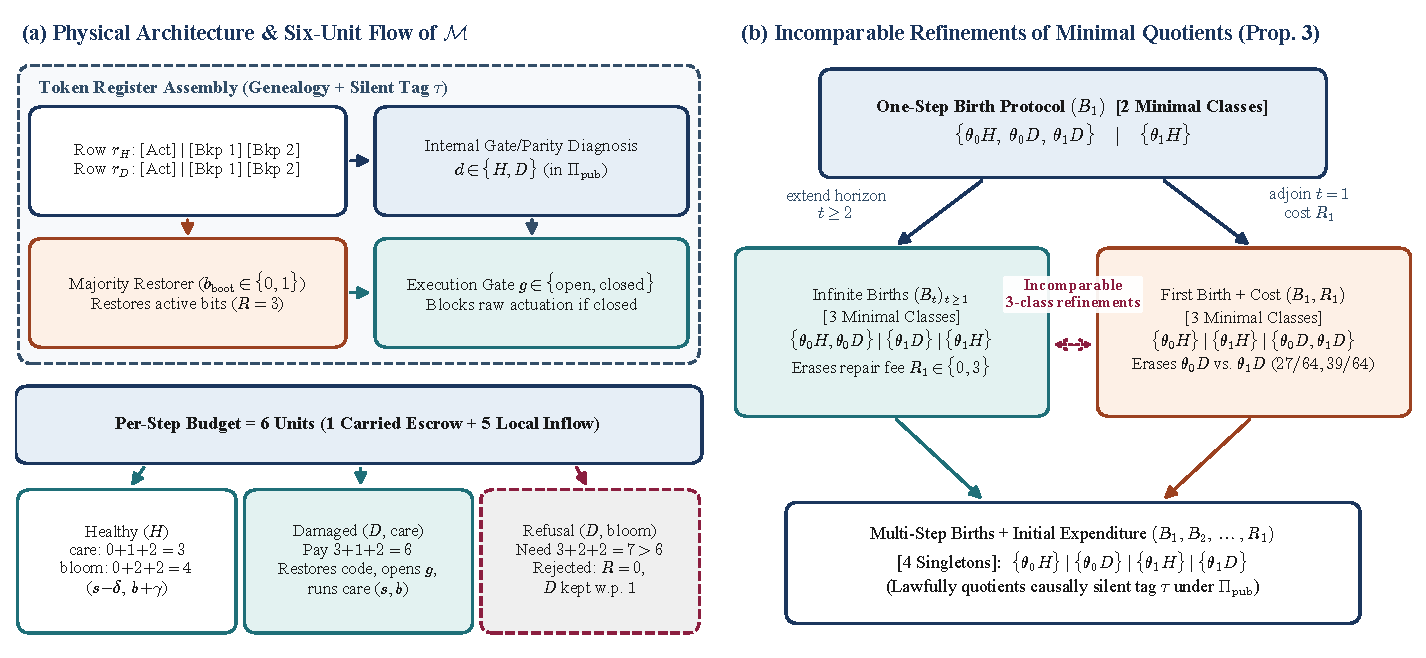
\includegraphics[width=0.99\linewidth,height=\textheight,keepaspectratio,alt={Physical
register architecture and predictive quotient lattice of the
regenerative process \textbackslash mathcal\{M\}. (a) Internal
three-cell instruction rows, parity/gate diagnostic, majority-vote
restorer, physical execution gate, and six-unit transaction paths. (b)
Non-monotonic diamond lattice of minimal predictive partitions across
four observation protocols (Proposition 3), showing two incomparable
three-class quotients.}]{figures/fig1_architecture_and_lattice.pdf}
\caption{Physical register architecture and predictive quotient lattice
of the regenerative process \(\mathcal{M}\). (a) Internal three-cell
instruction rows, parity/gate diagnostic, majority-vote restorer,
physical execution gate, and six-unit transaction paths. (b)
Non-monotonic diamond lattice of minimal predictive partitions across
four observation protocols (Proposition 3), showing two incomparable
three-class quotients.}
\end{figure}

\subsection{Lawful tag quotients versus von Neumann's
syntactic--constructor
gap}\label{lawful-tag-quotients-versus-von-neumanns-syntacticconstructor-gap}

Our preservation framework is not an indiscriminate plea for
microphysical maximalism. Within \(\mathcal{M}\), erasing the causally
silent physical tag \(\tau\) defines a non-injective projection
\(\pi_\tau\) that merges physically distinct raw tokens while
\emph{commuting exactly} with step transitions, six-unit budget
accounting, repair expenditures, genealogical parent/offspring labels,
and expected outcomes under every permitted public-history policy
(Proposition 4a, Appendix A.4). Eliminating \(\tau\) is a paradigm of
\emph{lawful explanatory compression}.

By contrast, two superficially plausible informational compressions fail
catastrophically. First, projecting a token onto its stored program
\(\theta\) while erasing its diagnostic state (\(H\) vs.~\(D\)) destroys
action affordability: \texttt{bloom} is feasible on \(H\) (\(4 \le 6\))
but rejected on \(D\) (\(7 > 6\)). Second, and more subtly, projecting a
token onto its \emph{decoded symbolic instruction}---the
majority-decoded bit pattern of its rows---while erasing the physical
gate variable \(g \in \{\mathrm{open}, \mathrm{closed}\}\) destroys raw
executable capacity (Proposition 4b). Two assemblies can carry
bit-for-bit identical decoded instructions
\(\theta_1 = (\mathrm{bloom}, \mathrm{care})\) under a healthy
diagnosis, yet the assembly with \(g = \mathrm{open}\) executes
\texttt{bloom} whereas the assembly with \(g = \mathrm{closed}\) is
physically blocked from actuation.

This provides a crisp stochastic realization of John von Neumann's
\citeyearpar{vonNeumann1966} foundational insight into self-reproducing
automata. Von Neumann showed that biological and computational
self-reproduction requires separating the \emph{passive syntactic
description} (tape \(I\), copied uninterpreted during replication) from
the \emph{active physical constructor} (mechanism \(A+B+C\), gated and
energized to translate instructions into causal work)
\citep{rosen1991, deacon2011}. Purely informational definitions of
agency or genetics that equate an organism's state with its decoded
sequence erase the physical enabling constraints---gates, polymerase
machinery, metabolic ATP budgets---that turn syntax into causal
execution. Microbial physiology illustrates both separations concretely:
in bacterial methyl-directed DNA mismatch repair, hemimethylated
template strands preserve backup sequence information while
ATP-consuming MutS--MutL--MutH complexes restore damaged active strands
and reopen stalled replisome progression; two daughter cells with
identical post-repair division distributions nevertheless differ in
depleted intracellular ATP reserves (\(R_1\)), and unmethylated sequence
identity without replisome gate clearance fails to support replication.

\section{Persistence, organizational closure, and diachronic
bearers}\label{persistence-organizational-closure-and-diachronic-bearers}

\subsection{Separating dynamical stability, cybernetic servocontrol, and
constraint
closure}\label{separating-dynamical-stability-cybernetic-servocontrol-and-constraint-closure}

A recurring temptation in systems theory and natural philosophy is to
search for a single topological or dynamical signature---such as a
closed phase-space orbit, non-trivial first homology \(H_1 \neq 0\), or
existence of an ergodic stationary density---that characterizes all
persistent objects \citep{friston2013}. Careful separation of dynamical,
cybernetic, and biological mechanisms shows why any such universal
signature conflates four fundamentally distinct modes of persistence
(Table 3).

First, \emph{passive dynamical invariance} requires neither topological
loops nor restorative work. Let \((\mathcal{X}, d)\) be a metric space
carrying a continuous semiflow \((\varphi_t)_{t \ge 0}\). Whenever a
forward orbit \(\{\varphi_t(x_0) : t \ge 0\}\) is precompact and
eventually resides inside a closed domain \(D \subseteq \mathcal{X}\),
its dynamical \(\omega\)-limit set
\(\omega(x_0) = \bigcap_{s \ge 0} \overline{\{\varphi_t(x_0) : t \ge s\}}\)
is non-empty, compact, and strictly \(\varphi\)-invariant. Yet on the
contractible Euclidean space \(\mathbb{R}^n\) (where
\(H_1(\mathbb{R}^n) = 0\)), the simple dissipative flow \(\dot{x} = -x\)
stays inside every closed ball around the origin and converges
monotonically to \(\omega(x_0) = \{0\}\) without any geometric cycle,
feedback sensor, or component replacement. Conversely, a frictionless
harmonic oscillator traces closed orbits with non-trivial loop topology
on its energy shell while performing zero self-repair if perturbed onto
a neighboring shell. Phase-space homology and attractor stability simply
do not track organizational self-maintenance.

\Needspace{16\baselineskip}

{\def\LTcaptype{none} % do not increment counter
\begin{longtable}[]{@{}
  >{\raggedright\arraybackslash}p{(\linewidth - 6\tabcolsep) * \real{0.2500}}
  >{\raggedright\arraybackslash}p{(\linewidth - 6\tabcolsep) * \real{0.2500}}
  >{\raggedright\arraybackslash}p{(\linewidth - 6\tabcolsep) * \real{0.2500}}
  >{\raggedright\arraybackslash}p{(\linewidth - 6\tabcolsep) * \real{0.2500}}@{}}
\toprule\noalign{}
\begin{minipage}[b]{\linewidth}\raggedright
Persistence Regime
\end{minipage} & \begin{minipage}[b]{\linewidth}\raggedright
Sustaining Mechanism
\end{minipage} & \begin{minipage}[b]{\linewidth}\raggedright
Counterfactual Signature under Structural Cut
\end{minipage} & \begin{minipage}[b]{\linewidth}\raggedright
Paradigm Literature
\end{minipage} \\
\midrule\noalign{}
\endhead
\bottomrule\noalign{}
\endlastfoot
1. Passive dynamical invariance & Conservative law or dissipative
potential (\(\dot{x}=-x\); crystal lattice) & Perturbation shifts orbit
or equilibrium; zero endogenous restoration of constraints & Topological
dynamics; classical mechanics \\
2. Externally scaffolded servocontrol & Fixed sensor--actuator negative
feedback regulating target variable & Regulates state variable, but
cutting sensor/heater triggers zero self-rebuild of hardware &
\citet{rosenblueth1943}; \citet{conantAshby1970} \\
3. Endogenous constraint closure & Work-coupled processes regenerate at
least one enabling constraint (\(g\), active code) & Survives bounded
internal damage via paid repair; fails under bootstrap/budget severance
& \citet{kant1790}; \citet{varela1974}; \citet{rosen1991};
\citet{montevilMossio2015} \\
4. Adaptive / finite-memory viability & History-sensitive policy shifts
modes to remain inside viability kernel \(K^\star\) & Modulates
behavioral trajectory before lethal boundary contact; separates
\(m \ge 1\) from \(m=0\) & \citet{aubinCellina1984};
\citet{diPaolo2005}; \citet{bich2024} \\
\end{longtable}
}

Table 3. Four non-equivalent regimes of temporal persistence. Neither
dynamical attraction (Regime 1) nor fixed servocontrol (Regime 2)
entails endogenous constraint regeneration (Regime 3) or
history-sensitive adaptive viability (Regime 4).

Second, \emph{externally scaffolded cybernetic servocontrol}
\citep{rosenblueth1943, conantAshby1970} introduces genuine
error-correcting feedback: a thermostat or Watt governor senses
deviations of room temperature or shaft speed from a reference range and
actuates a compensating response. By Conant and Ashby's
\citeyearpar{conantAshby1970} Good Regulator principle, effective
disturbance rejection constrains the controller's mapping from
disturbances to actions. Yet in an ordinary servomechanism, every
physical constraint of the controller itself---its bimetallic strip,
wiring, and casing---is externally manufactured and passively endures on
a slower timescale. The thermostat regulates \emph{room temperature}; it
does nothing to regenerate \emph{itself}.

Third, \emph{organizational constraint closure}---rooted in Kant's
\citeyearpar[§§64--65]{kant1790} analysis of \emph{Naturzwecke} as
beings in which parts reciprocally produce and maintain one another, and
developed through autopoiesis
\citep{varela1974, maturanaVarela1980, weberVarela2002},
\((M,R)\)-systems \citep{rosen1991}, autocatalytic work--constraint
cycles \citep{kauffman1993, deacon2011}, and closure of constraints
\citep{montevilMossio2015}---requires a stricter constitutive loop. A
collection of constraints \(\mathcal{C} = \{c_1, \dots, c_k\}\) exhibits
constraint closure when the thermodynamic or informational processes
channeled by \(c_i\) actively regenerate or repair at least one other
enabling constraint \(c_j\) that would otherwise degrade on the
timescale of inquiry \citep{jonas1966, thompson2007}. Our regenerative
model \(\mathcal{M}\) captures a minimal, fully transparent instance of
this third regime without pretending to total autopoietic self-creation:
its active instruction cells and execution gate \(g\) are enabling
constraints on future metabolic action that suffer stochastic
degradation (\(q > 0\)) and are physically reconstructed from internal
backups using budgeted energetic inflow, while still relying on trusted
primitives (\(b_{\mathrm{boot}}\), environmental supply).

Fourth, as \citet{diPaolo2005} demonstrated in critiquing binary
autopoiesis (where an organization either persists or dies without
gradation), genuine agency requires \emph{adaptivity}: the capacity to
monitor graded proximity to viability boundaries
\citep{aubinCellina1984} and modulate internal or interactive modes
accordingly \citep{barandiaran2009, bich2024}.

\subsection{Interventional vulnerability, finite-memory viability, and
fixed-sample
limits}\label{interventional-vulnerability-finite-memory-viability-and-fixed-sample-limits}

How should organizational dependence be tested without sneaking
universal topological assumptions through the back door? Fix a target
capability certificate \(\mathcal{C}\) over a horizon \(T\) (for
example, positive probability of restored execution) and a declared
repertoire \(\mathcal{I}\) of structural component deletions
\(D \subseteq \mathcal{E}\) \citep{woodward2003, craver2007}. Let
\(\mathcal{F}(\mathcal{C}, \mathcal{I}) \subseteq \mathcal{P}_{\mathrm{fin}}(\mathcal{E})\)
denote the family of finite deletion sets under which \(\mathcal{C}\)
fails.

\textbf{Proposition 5 (Minimal interventional cut-set reconstruction).}
\emph{Suppose failure of \(\mathcal{C}\) is monotone with respect to
deletions in \(\mathcal{I}\) (if \(D \in \mathcal{F}\) and
\(D \subseteq D'\), then \(D' \in \mathcal{F}\)). Then
\(\mathcal{F}(\mathcal{C}, \mathcal{I})\) is uniquely determined by its
antichain of inclusion-minimal destructive cut-sets
\(\mathcal{V}_{\min}(\mathcal{C}, \mathcal{I})\): a finite deletion
\(D\) destroys \(\mathcal{C}\) if and only if \(M \subseteq D\) for some
\(M \in \mathcal{V}_{\min}(\mathcal{C}, \mathcal{I})\).}

Proposition 5 (proved in Appendix A.2) turns organizational integrity
into a crisp interventional hypergraph while exposing three crucial
caveats. First, monotonicity is a substantive causal hypothesis, not a
logical truism: in biological networks with inhibitory pathways or
latent backups, ablating an inhibitor can \emph{restore} a blocked
function, violating monotonicity. Second, \(\mathcal{V}_{\min}\) is
indexed to \(\mathcal{I}\): if allowed interventions perturb only a
causally decoupled variable \(u\) while capability \(q(x,u) = x\)
depends solely on \(x\), then \(\mathcal{V}_{\min} = \emptyset\)---not
because the system is indestructible, but because the test repertoire
missed its causal support. Third, one must distinguish \emph{erasing
observational readout access} from \emph{destroying the underlying
mechanism}: cutting a telemetry wire blinds the observer's certificate
while leaving endogenous repair intact.

In \(\mathcal{M}\), interventional ablations isolate three distinct
enabling conditions for self-repair: \emph{(i) cutting the bootstrap
unit} (\(b_{\mathrm{boot}} = 0\)) leaves backups and funds intact but
blocks internal restoration; \emph{(ii) clamping the repair-stage
balance to \(2 < 3\) units} leaves hardware intact but starves paid
restoration; and \emph{(iii) erasing all three cells of both rows}
destroys the conserved mutual information \citep{coverThomas2006} so
that no deterministic decoder can recover both \(\theta_0\) and
\(\theta_1\) from the post-damage state. None of these failures can be
diagnosed from passive output histories prior to perturbation.

Two further mathematical results---formalized in Proposition 6 (proved
in Appendix A.2)---reveal why maintaining viability in partially
observed environments outstrips memoryless reactivity and finite
black-box sampling:

\textbf{Proposition 6 (Finite-memory viability separation and
fixed-sample risk impossibility).} \emph{(a) Let
\(K^\star = \operatorname{gfp}(F_S) \subseteq \mathcal{X}\) be the
maximal viable state kernel of a finite controlled transition system
inside a safe set \(S \subseteq \mathcal{X}\), where
\(F_S(U) = \{x \in S : \exists a \in \mathcal{A},\ \mathrm{supp}\,T(\cdot \mid x,a) \subseteq U\}\).
Even though \(K^\star\) is a subset of states, under partial observation
\(h: \mathcal{X} \to \mathcal{O}\) there exist five-state systems in
which \textbf{every} memoryless observation policy
\(\pi_0: \mathcal{O} \to \mathcal{A}\) exits \(S\) within two steps with
probability \(1/2\), whereas a \textbf{one-step finite-memory
controller} \(\pi_1: \mathcal{O} \times \mathcal{O} \to \mathcal{A}\)
maintains perpetual viability
\(\mathbb{P}_{\pi_1}(X_t \in K^\star\ \forall t \ge 0) = 1\).} \emph{(b)
Fix any finite sample size \(n \ge 1\) and significance level
\(\alpha \in [0, 1)\). Let
\(\psi: \{0,1\}^n \to \{\mathrm{certify}, \mathrm{reject}\}\) be any
statistical rule observing \(n\) independent indicator draws of
out-of-support violation events \(Z_i \sim \mathrm{Bernoulli}(r)\). If
\(\psi\) respects the zero-violation soundness bound
\(\mathbb{P}_r(\psi = \mathrm{certify}) \le \alpha\) for all positive
violation rates \(r \in (0,1]\), then by continuity
\(\mathbb{P}_0(\psi = \mathrm{certify}) \le \alpha\); conversely, no
fixed-\(n\) black-box test can certify \(r = 0\) with high probability
\((1-\beta > \alpha)\) while uniformly bounding false certification
across arbitrarily small positive hazard rates \(r = \varepsilon > 0\)
\citep{leCam1973, mayo2018}.}

Philosophically, Proposition 6 closes two major loopholes. Part (a),
illustrated in Figure 2a, shows why internal memory
registers---extending an agent's effective horizon beyond instantaneous
sensory surfaces
\citep{sethTsakiris2018, kaelbling1998, papadimitriouTsitsiklis1987}---can
be \emph{constitutively necessary} for viable persistence even when the
underlying safe region \(K^\star\) is state-defined. Part (b) proves why
purely inductive, model-free prediction from a finite training sample
cannot by itself certify strict structural safety or organizational
closure: without mechanistic prior bounds on transition support,
arbitrarily small unvisited failure modes remain statistically
indistinguishable from zero risk over \(n\) trials.

\subsection{Token persistence, genealogical lineages, and symmetrical
fission}\label{token-persistence-genealogical-lineages-and-symmetrical-fission}

Even when physical restoration and viability are established,
\emph{whose} persistence has been explained? Processual and
immunological philosophers of biology rightly emphasize that organisms
persist through continuous metabolic and cellular turnover rather than
static material identity
\citep{whitehead1929, pradeu2012, dupreNicholson2018}, while
evolutionary theorists show that biological individuality splinters
across physiological, immunological, and Darwinian selection criteria
\citep{clarke2010, godfreySmith2009, maynardSmithSzathmary1995}.

Our regenerative process \(\mathcal{M}\) makes this split formally
explicit by recording \emph{parental token retention} and \emph{strict
offspring birth} as distinct causal events. When a healthy
\(\theta_0 H\) founder survives with probability \(s\) and produces a
healthy newborn with probability \(b(1-q)\), the retained parent and the
newborn subsequently possess identical physical registers, identical
predictive classes, and identical forward capabilities. Yet they are
numerically distinct tokens with distinct causal histories: one
continued an existing metabolic trajectory; the other originated in a
reproductive branching event \citep{wiggins2001}.

Symmetrical fission sharpens the boundary of purely causal criteria
\citep{parfit1984}. Suppose an amoeba or duplicator divides cleanly into
two daughters \(y_1, y_2\), each equally causally and informationally
continuous with the predecessor \(x\). Because \(y_1 \neq y_2\),
numerical identity---which is symmetric and transitive---cannot hold
between \(x\) and both daughters. Any theory must choose among three
conventions: selecting a privileged continuation (asymmetrical
parent/bud convention, as in \(\mathcal{M}\)), holding that \(x\) ceases
to exist at division while initiating two new tokens (clonal binary
fission), or shifting the explanatory bearer from an individual token to
a \emph{genealogical lineage}. Predictive equivalence across future
outputs is completely silent among these three options.

Furthermore, conditioning a branching or absorbing Markov process on
long-run non-extinction alters its probability law in a mathematically
subtle way that teleological theories often misread. For an absorbing
chain on a transient viable set, the \emph{quasi-stationary
distribution} (QSD) \(q\)---the limiting state distribution
\(\lim_{t\to\infty} \mathbb{P}(X_t \in \cdot \mid \tau_{\mathrm{ext}} > t)\)
among trajectories still alive at \(t\)---differs strictly in general
from the stationary law \(\varpi(x) \propto q(x) h(x)\) of the
\emph{Doob \(h\)-transformed survivor process} conditioned on surviving
forever, weighted by reproductive or survival value \(h(x)\)
\citep{doob1957, darrochSeneta1965, collet2013}. In \(\mathcal{M}\)'s
marked genealogy, weighting lineages by reproductive value yields a
valid statistical many-to-one identity across ancestral paths, yet that
reweighted kernel neither represents uniform sampling of living
individuals nor defines a causally executable policy available to a
single body. As \citet{cuciniello2026} observes, organizational
teleology cannot slide from maintaining a present token to preserving a
cross-generational form without accounting for this shift of diachronic
bearer.

\section{Optimization, bearer divergence, and the grounds of
purpose}\label{optimization-bearer-divergence-and-the-grounds-of-purpose}

\subsection{Underdetermination of evaluation: reward shaping,
dual-criterion gauge, and rank
obstructions}\label{underdetermination-of-evaluation-reward-shaping-dual-criterion-gauge-and-rank-obstructions}

Turn now from objecthood to our second overarching question: when does a
successful representation of a system's dynamics justify claiming that
an activity occurs \emph{for} an outcome? A pervasive strategy in
decision theory, behavioral ecology, and cognitive science is
\emph{optimality attribution}: exhibit a scalar reward, utility, or
free-energy functional under which the system's observed behavior is
optimal \citep{puterman1994, friston2010}. Four formal obstructions show
why behavioral optimization, taken alone, never identifies an endogenous
purpose.

First, \emph{inverse optimality is massively underdetermined}. As
\citet[3.1]{ngRussell2000} established for Markov decision processes,
any observed policy is trivially optimal under the constant zero reward,
and in discounted dynamic programming \citep{blackwell1965} adding any
potential-based shaping term
\(r'(x,a,x') = r(x,a,x') + \beta \psi(x') - \psi(x)\) leaves the set of
optimal policies completely invariant while altering state valuations
arbitrarily. Even more starkly, fixing a set of physically feasible
transitions and bare observational evidence leaves opposite evaluative
rankings over initial actions logically compatible unless an independent
functional or historical premise constrains the objective.

Second, \emph{preferences and viability constraints need not admit any
scalar representation}. Classic representational measurement theory
proves that numerical utility exists only under completeness,
transitivity, and Archimedean continuity axioms \citep{krantz1971}. When
an organism or institution faces genuinely incomparable multidimensional
survival and epistemic constraints---a non-total preorder over
admissible trajectories---no real-valued scalar objective preserves both
strict improvements and genuine incomparabilities. Even where a scalar
criterion exists, optimal control defines a \emph{set-valued
correspondence} \(\mathcal{A}^\star(z) \subseteq \mathcal{A}\) rather
than a unique direction: at exact price-and-discount thresholds, active
repair and passive idling tie strictly.

Third, \emph{combined resource--information functionals suffer affine
gauge non-identifiability and local rank obstructions}. Many unified
theories of agency---including active inference's expected free energy,
which combines pragmatic/extrinsic value with epistemic/intrinsic
information gain \citep{parrPezzuloFriston2022}, and
thermodynamic--informational trade-offs---postulate a composite
objective \(J = R - \lambda I\) balancing a physical or metabolic return
\(R\) against an informational functional \(I\) at trade-off rate
\(\lambda > 0\). (Note that \(I\) here denotes task-specific uncertainty
or information cost, not Tononi's \citeyearpar{tononi2004}
causal-partition integrated information \(\Phi^{\mathrm{IIT}}\), which
measures irreducible whole-over-parts cause--effect repertoire
structure.) Whenever downstream behavior or model selection depends only
on the composite score \(J\), the affine gauge transformation

\[R' = R + \lambda \chi, \qquad I' = I + \chi\]

leaves \(J' = R' - \lambda I' = J\) identically unchanged for any state
function \(\chi\): observing composite optimality cannot disentangle
metabolic drive from epistemic drive without independent physical and
informational anchors. Worse still, one cannot assume that
multidimensional behavioral responses always factor smoothly through a
universal two-axis \((R, I)\) bottleneck:

\textbf{Proposition 7 (Local rank-three obstruction to universal smooth
two-axis factorization).} \emph{In the regenerative process
\(\mathcal{M}\) under autonomous
\(\theta_0 = (\mathrm{care},\mathrm{care})\) execution from a healthy
state with fixed \((\delta, \gamma)\), consider the observable one-step
response map \(\Psi(s, b, q) := (s,\, b,\, bq)\) recording parental
retention probability, strict-birth probability, and joint probability
of birth with damaged offspring over the open parameter domain
\(U = \{(s,b,q) : 0 < \delta < s < 1,\ 0 < b < 1-\gamma,\ 0 < q < 1\}\).
The Jacobian matrix \(D\Psi(s,b,q)\) has determinant
\(\det D\Psi(s,b,q) = b > 0\) everywhere on \(U\). By the chain rule,
\(\Psi\) cannot factor on any non-empty open subset of \(U\) as
\(g \circ f\) through \(C^1\) maps \(f: U \to \mathbb{R}^2\) and
\(g: \mathbb{R}^2 \to \mathbb{R}^3\).}

Proposition 7 (proved in Appendix A.3) blocks any attempt to treat
two-dimensional resource--information coordinates as an a priori
universal bottleneck for organized processes.

\subsection{Exact growth ceiling, joint realization, and
organism--lineage
conflict}\label{exact-growth-ceiling-joint-realization-and-organismlineage-conflict}

What happens, instead, when we derive demographic performance
\emph{directly from the physical transactions, six-unit budget, and
hereditary code} of \(\mathcal{M}\) rather than fitting an ex post
reward? Recall from Table 1 that one-step expected total output
(retained parent plus strict newborn) is \(k_c := s + b\) under
\texttt{care} and \(k_b := s - \delta + b + \gamma\) under
\texttt{bloom}. Because each surviving or newborn token enters the next
census damaged with probability \(q\) (where repair forces
\texttt{care}) and healthy with probability \(1-q\), the two hereditary
programs \(\theta_0 = (\mathrm{care},\mathrm{care})\) and
\(\theta_1 = (\mathrm{bloom},\mathrm{care})\) carry intrinsic per-capita
multiplication rates

\[\lambda_0 := k_c = s + b, \qquad \lambda_1 := (1 - q) k_b + q k_c.\]

Let \(\Pi_{\mathrm{pub}}\) denote the full class of \emph{admissible
public-history policies}: at each census \(t\), the controller may use
the entire observable history of diagnoses, public transaction receipts,
and population counts---together with arbitrary joint randomization
across living tokens---to issue action requests (\texttt{care},
\texttt{bloom}, \texttt{stop}), but may \emph{not} peek at
contemporaneous actuation/damage noise before acting or read causally
silent tags. Each living token at census \(t\) occupies an independent
local six-unit resource site (\(1\) carried escrow unit plus \(5\) local
inflow units), contrasting open per-capita resource regimes with
globally capped finite habitats where exponential branching
\(\rho_* > 1\) is bounded by carrying capacity. Let \(N_t\) denote total
living population size at census \(t\).

\textbf{Theorem 1 (Full-policy expected growth ceiling and same-process
joint realization).} \emph{Fix any parameter vector
\((s,\delta,b,\gamma,q)\) in the strict probabilistic domain of Table 1
and any finite non-empty canonical initial population \(P_0\). Define}

\[\rho_* := \max\{1,\, \lambda_0,\, \lambda_1\}.\]

\begin{enumerate}
\def\labelenumi{\arabic{enumi}.}
\tightlist
\item
  \textbf{Uniform upper ceiling and optimality.} \emph{There exists a
  finite constant \(C > 0\) (depending only on the parameters and
  \(P_0\), independent of \(\pi\) and \(t\)) such that
  \(\mathbb{E}_\pi[N_t] \le C \rho_*^t\) for every admissible policy
  \(\pi \in \Pi_{\mathrm{pub}}\) and every finite census \(t \ge 0\).
  Moreover, an explicit stationary policy achieves two-sided bounds
  \(c_1 \rho_*^t \le \mathbb{E}[N_t] \le c_2 \rho_*^t\) (\(c_1 > 0\)),
  so \(\rho_*\) is the least positive uniform exponential upper base
  across \(\Pi_{\mathrm{pub}}\).}
\item
  \textbf{Exact same-process joint realization from a damaged founder.}
  \emph{Starting from a single damaged founder carrying stored program
  \(\theta_i\) (\(i \in \{0,1\}\)), paid majority-vote physical
  restoration (\(R_1 = 3\)), gate-mediated internal execution of the
  restored code, faithful hereditary transmission, and two-sided
  attainment of the full-policy growth ceiling \(\rho_*\) hold
  \textbf{jointly in \(\mathcal{M}\)} if and only if:}
\end{enumerate}

\[\begin{aligned}
\theta_0\text{ repairs and attains }\rho_* &\iff \gamma \le \delta \ \text{and}\ k_c \ge 1,\\
\theta_1\text{ repairs and attains }\rho_* &\iff \gamma \ge \delta \ \text{and}\ \lambda_1 \ge 1.
\end{aligned}\]

Theorem 1 (proved in Appendix A.5) delivers both our constructive
compatibility benchmark and three sharp philosophical separations
concerning purpose and persistence:

First, \emph{implementation semantics shape what counts as optimal}
(Figure 2b). Why does the constant \(1\) appear inside
\(\rho_* = \max\{1, \lambda_0, \lambda_1\}\)? Because in subcritical
environments where both \(\lambda_0 < 1\) and \(\lambda_1 < 1\) (Regime
I of Figure 2b), repeatedly submitting the unaffordable \texttt{bloom}
request on a damaged token triggers transaction rejection, preserving
that single token without actuation noise
(\(N_t \equiv 1 = 1^t\))---analogous to metabolically dormant bacterial
persister cells surviving antibiotic or starvation regimes that drive
actively dividing phenotypes (\(\lambda_0, \lambda_1 < 1\)) toward
extinction, whereas iteroparous maintenance (\texttt{care}, Regime II)
and semelparous or high-fecundity proliferative investment
(\texttt{bloom}, Regime III) dominate distinct ecological regions. Far
from asserting a universal law that inactivity prevents decay, Regime I
exposes how optimal-control conclusions depend on the physical semantics
of arrested actuation: if rejected requests suffered background
attrition, the unit floor would vanish.

\begin{figure}
\centering
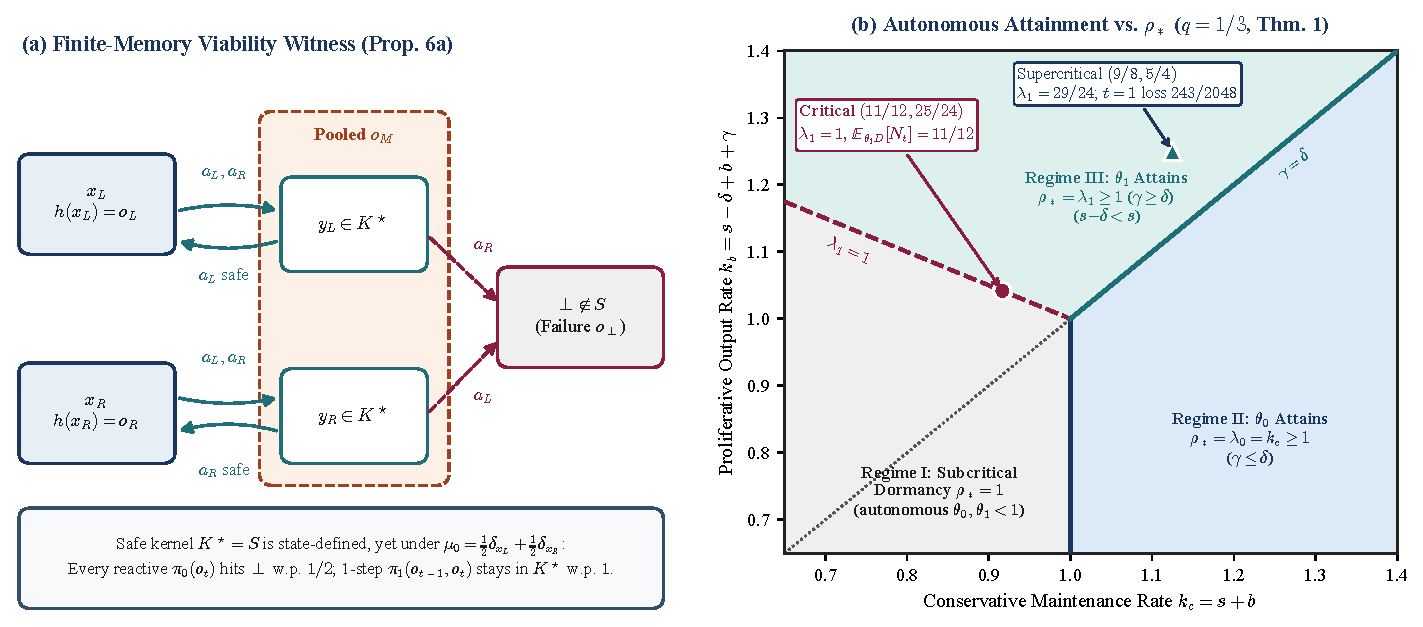
\includegraphics[width=0.99\linewidth,height=\textheight,keepaspectratio,alt={Finite-memory
viability separation and full-policy demographic phase diagram. (a)
Five-state partially observed viability witness (Proposition 6a) in
which observation pooling h(y\_L)=h(y\_R)=o\_M forces every reactive
policy \textbackslash pi\_0(o\_t) into two-step failure with probability
1/2 while one-step memory \textbackslash pi\_1(o\_\{t-1\},o\_t)
maintains perpetual viability in K\^{}\textbackslash star. (b) Exact
(k\_c, k\_b) attainment phase diagram at damage rate q = 1/3 (Theorem
1), showing the subcritical refusal/dormancy floor (\textbackslash
rho\_*=1), conservative maintenance attainment (\textbackslash
theta\_0), proliferative attainment (\textbackslash theta\_1), and the
critical (11/12, 25/24) and supercritical (9/8, 5/4) rational
witnesses.}]{figures/fig2_memory_and_phase.pdf}
\caption{Finite-memory viability separation and full-policy demographic
phase diagram. (a) Five-state partially observed viability witness
(Proposition 6a) in which observation pooling \(h(y_L)=h(y_R)=o_M\)
forces every reactive policy \(\pi_0(o_t)\) into two-step failure with
probability \(1/2\) while one-step memory \(\pi_1(o_{t-1},o_t)\)
maintains perpetual viability in \(K^\star\). (b) Exact \((k_c, k_b)\)
attainment phase diagram at damage rate \(q = 1/3\) (Theorem 1), showing
the subcritical refusal/dormancy floor (\(\rho_*=1\)), conservative
maintenance attainment (\(\theta_0\)), proliferative attainment
(\(\theta_1\)), and the critical \((11/12, 25/24)\) and supercritical
\((9/8, 5/4)\) rational witnesses.}
\end{figure}

Second, \emph{proliferative optimization splits the organism from the
lineage}. Whenever \(\gamma > \delta > 0\) and \(\lambda_1 \ge 1\),
Theorem 1 certifies that \(\theta_1\) uniquely attains
\(\rho_* = \lambda_1 > \lambda_0\). Yet on every healthy token,
executing \texttt{bloom} \emph{strictly reduces} that individual's
one-step survival probability from \(s\) to \(s - \delta\) in exchange
for raising strict births from \(b\) to \(b + \gamma\). What maximizes
expected lineage proliferation actively endangers the individual
organism performing it. This furnishes an exact mechanistic counterpart
to multilevel selection theory
\citep{okasha2006, maynardSmithSzathmary1995} and to Garson's
\citeyearpar{garson2019} crucial distinction between \emph{differential
retention} (persisting longer as the same token) and \emph{differential
reproduction} (multiplying copies). Calling \texttt{bloom} ``adaptive
for persistence'' without indexing the bearer conflates two opposing
causal tendencies.

Third, \emph{asymptotic growth rates diverge from both finite-deadline
expectations and single-population stochastic survival}. Evaluate
\(\mathcal{M}\) at the critical rational point
\((s,\delta,b,\gamma,q) = (2/3, 1/8, 1/4, 1/4, 1/3)\). Here
\(k_c = 11/12\), \(k_b = 25/24\), and
\(\lambda_1 = \frac{2}{3}\cdot\frac{25}{24} + \frac{1}{3}\cdot\frac{11}{12} = 1 = \rho_*\).
Starting from a damaged \(\theta_1 D\) founder (which must repair and
run \texttt{care} at \(t=1\)), expected population size is
\(\mathbb{E}_{\theta_1}[N_t] = 11/12 < 1\) at \emph{every} positive
census \(t \ge 1\), whereas repeated transaction refusal maintains
\(N_t = 1\) on every path---even though both share the exact asymptotic
exponential base \(\rho_* = 1\). Moreover, even in the strictly
supercritical regime \((3/4, 1/8, 3/8, 1/4, 1/3)\) where
\(\lambda_1 = 29/24 > \lambda_0 = 9/8 > 1\), starting two independent
healthy founders (\(\theta_1 H\) and \(\theta_0 H\)) yields an exact
first-census event of probability
\((1 - (s-\delta))(1 - (b+\gamma))(1 - (1-s)(1-b)) = \frac{3}{8}\cdot\frac{3}{8}\cdot\frac{27}{32} = 243/2048 \approx 0.1187\)
in which \emph{the higher-growth \(\theta_1\) lineage goes completely
extinct at \(t=1\) while the slower \(\theta_0\) lineage survives}. At
that same first census, the unconditional expected \(\theta_1\)-share
(setting \(0/0 := 0\)) is \(2095/4096 \approx 0.5115\), the share
conditioned on non-extinction is \(2095/4006 \approx 0.5230\), and the
ratio of expected counts \(\mathbb{E}[N_1^{(1)}]/\mathbb{E}[N_1]\) is
\(10/19 \approx 0.5263\) \citep{price1970, athreyaNey1972}. High
expected growth guarantees neither pathwise victory in one finite
population nor interchangeability of expectations and ratios;
probabilistic selection requires explicit quantification over a finite
horizon \(T\) and \(n\) independent cohorts.

\subsection{Four stratified grounds of purpose and the normativity
challenge}\label{four-stratified-grounds-of-purpose-and-the-normativity-challenge}

How, then, are functional and purposive attributions legitimately
grounded? In classical philosophy of biology, Cummins's
\citeyearpar{cummins1975} \emph{causal-role analysis} explains how a
part contributes to a system-level capacity, whereas
\emph{selected-effects theories}
\citep{wright1973, millikan1984, neander1991, godfreySmith1994} explain
\emph{why} the part exists via ancestral selection---grounding
malfunction norms at the price of rendering de novo homeostatic traits
epiphenomenal (``swampman'' cases). Seeking an ahistorical yet normative
third way, \emph{organizational accounts}
\citep{mossio2009, montevilMossio2015} ground a trait's function in its
contribution to maintaining a closed regime of constraints on which the
trait's own existence depends, recently enriched by Bich's
\citeyearpar{bich2024} regulatory-control criterion and scrutinized by
\citet{corti2023} and \citet{cuciniello2026}.

Corti's \citeyearpar[§3]{corti2023} critique cuts to the heart of
organizational teleology---echoing Bedau's \citeyearpar{bedau1992}
challenge regarding telic value and Davies's \citeyearpar{davies2001}
causal-role deflationism: \emph{why does the purely causal fact that a
closed system will cease to exist unless component \(C\) performs
activity \(A\) generate an objective biological norm that \(C\)
\textbf{ought} to perform \(A\) (so that failure counts as genuine
malfunction rather than mere state transition)?} Dismissing Corti's
objection by saying ``biological functions do not entail moral
obligations'' misses his target: Corti challenges \emph{intrinsic
biological functional correctness} itself, not just ethics.

Our preservation and bearer-indexing framework resolves this impasse not
by postulating a magical derivation of categorical oughts from bare
causal loops, but by \emph{stratifying four distinct evidential grounds}
that teleological language conflates (Table 4):

\Needspace{16\baselineskip}

{\def\LTcaptype{none} % do not increment counter
\begin{longtable}[]{@{}
  >{\raggedright\arraybackslash}p{(\linewidth - 6\tabcolsep) * \real{0.2500}}
  >{\raggedright\arraybackslash}p{(\linewidth - 6\tabcolsep) * \real{0.2500}}
  >{\raggedright\arraybackslash}p{(\linewidth - 6\tabcolsep) * \real{0.2500}}
  >{\raggedright\arraybackslash}p{(\linewidth - 6\tabcolsep) * \real{0.2500}}@{}}
\toprule\noalign{}
\begin{minipage}[b]{\linewidth}\raggedright
Rung
\end{minipage} & \begin{minipage}[b]{\linewidth}\raggedright
Ground of Attribution
\end{minipage} & \begin{minipage}[b]{\linewidth}\raggedright
Required Bearer \& Evidence Beyond Output Fit
\end{minipage} & \begin{minipage}[b]{\linewidth}\raggedright
Normative Force Licensed (and Limit)
\end{minipage} \\
\midrule\noalign{}
\endhead
\bottomrule\noalign{}
\endlastfoot
\textbf{1. Systemic causal role} & Constitutive decomposition
\citep{cummins1975, craver2007} & Specified host capacity \(\Psi\);
interventional ablation shows \(C\)'s activity contributes to \(\Psi\) &
\emph{Explanatory relevance} relative to chosen \(\Psi\); \textbf{no}
intrinsic malfunction norm \citep{davies2001} \\
\textbf{2. Endogenous regulatory \& viability closure} &
Self-maintaining constraint + error-sensitive control
\citep{nagel1977, mossio2009, diPaolo2005, bich2024} & Diachronic token;
state-sensitive gate/repair counters perturbations to viable kernel
\(K^\star\) & \emph{System-conditional viability standard}
(success/failure relative to maintaining \emph{this} closure);
\textbf{not} categorical value \\
\textbf{3. Selective / retention etiology} & Differential reproduction
or differential retention \citep{wright1973, millikan1984, garson2019} &
Lineage or plastic repertoire; historical covariance explains current
prevalence of trait \(\theta\) & \emph{Historical proper-function
standard} (malfunction vs.~ancestral selection regime); can
\textbf{conflict} with Rung 2 \\
\textbf{4. Reflective practical / moral reason} & Deliberative
endorsement \& interpersonal justification
\citep{korsgaard1996, scanlon1998, list2019} & Reflective agent /
institution; reasons survive normative scrutiny beyond sheer persistence
\citep{street2006} & \emph{Categorical / justificatory normativity};
\textbf{never} entailed by Rungs 1--3 alone \\
\end{longtable}
}

Table 4. Four stratified, non-interchangeable grounds of functional and
purposive explanation. Advancing from a lower rung to a higher rung
requires explicit new structural, historical, or deliberative evidence.

Look at what Table 4 clarifies about both Corti's challenge and our
regenerative model \(\mathcal{M}\):

\begin{enumerate}
\def\labelenumi{\arabic{enumi}.}
\tightlist
\item
  \textbf{Meeting Corti and Bedau honestly at Rung 2.} \citet{corti2023}
  is entirely right that \emph{mere existential dependence} does not
  yield \emph{unconditional or categorical} normativity: a
  self-sustaining hurricane or autocatalytic toxin has no unconditional
  claim to persist, and if a perturbation shifts a closed network into a
  \emph{different} stable regime, static closure alone cannot say
  whether the shift is ``malfunction'' or ``innovation''
  \citep[§§4--6]{cuciniello2026}. What Rung 2 \emph{does}
  establish---when constraint closure is paired with dedicated
  state-sensitive regulatory architecture
  \citep{nagel1977, diPaolo2005, bich2024, walsh2015}---is an
  \emph{objective counterfactual asymmetry internal to the system's
  viability}: in \(\mathcal{M}\), the diagnostic sensor, majority-vote
  restorer, and execution gate \(g\) exist specifically in a causal
  configuration that detects departures from intact rows and expends
  three resource units to reinstate the pre-damage code. In an
  engineered realization of \(\mathcal{M}\), that reference standard is
  fixed by explicit construction design; in a living cell's DNA
  mismatch-repair pathway, that reference standard is stabilized jointly
  by Rung 2 regulatory architecture and Rung 3 selective history.
  Neither requires smuggling categorical value into physics
  \citep{bedau1992}.
\item
  \textbf{Why Rung 2 and Rung 3 cannot be collapsed---and why bearer
  indexing reconciles them.} Because healthy \texttt{bloom} degrades
  Rung 2 token viability (\(s - \delta < s\)) while advancing Rung 3
  lineage selection (\(\lambda_1 > \lambda_0\)), organizational
  teleology (Rung 2) and evolutionary selected-effects teleology (Rung
  3) are \emph{not rival definitions of a single relation}. They answer
  purposive questions indexed to \emph{different bearers} (the
  physiological organism vs.~the Darwinian lineage;
  \citet{godfreySmith2009}) or \emph{different retention processes}
  (synchronic persistence vs.~neural/ecological differential retention;
  \citet{garson2019}). By contrast, \(\mathcal{M}\)'s growth rate
  \(\rho_*\) in isolation---prior to cohort selection history (Rung 3)
  or internal representation of population size (which tokens in
  \(\mathcal{M}\) wholly lack)---is a \emph{demographic performance
  metric}, not an intrinsic intention of the individual body.
\item
  \textbf{Protecting Rung 4 autonomy from evolutionary and institutional
  survivalism.} Even when Rungs 1--3 all align---as in a
  self-reproducing social institution or evolved behavioral
  disposition---persisting or out-reproducing rivals never automatically
  generates a Rung 4 practical or moral reason to endorse that
  persistence \citep{korsgaard1996, street2006, scanlon1998}. Predatory
  institutions can exhibit formidable constraint closure; autonomous
  agents can reflectively sacrifice individual or lineage survival for
  justified commitments \citep{list2019} (Figure 3).
\end{enumerate}

\begin{figure}
\centering
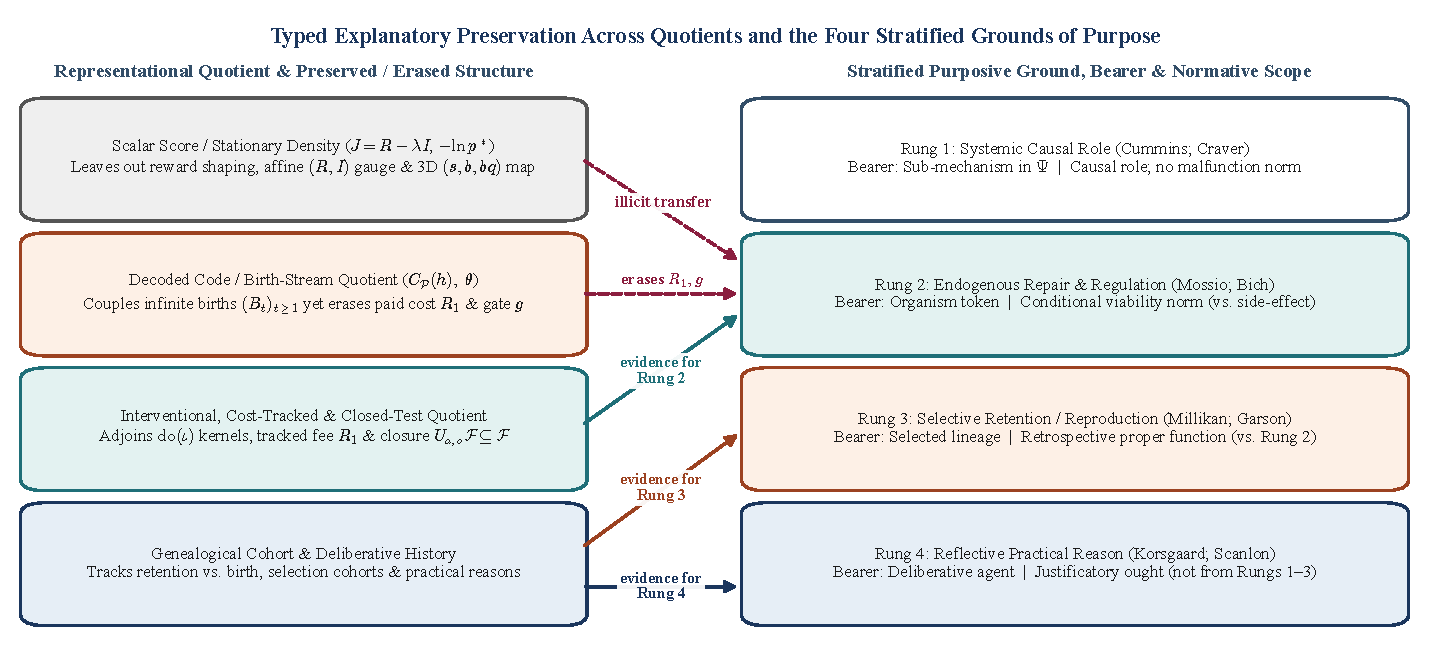
\includegraphics[width=0.99\linewidth,height=\textheight,keepaspectratio,alt={Summary
of typed explanatory preservation across representational quotients
(left) and its alignment with the four stratified grounds of functional
and purposive attribution (right), highlighting required invariance
bridges versus illicit cross-bearer
transfers.}]{figures/fig3_preservation_and_rungs.pdf}
\caption{Summary of typed explanatory preservation across
representational quotients (left) and its alignment with the four
stratified grounds of functional and purposive attribution (right),
highlighting required invariance bridges versus illicit cross-bearer
transfers.}
\end{figure}

\section{Explanatory discipline, competitor diagnostics, and testable
discriminations}\label{explanatory-discipline-competitor-diagnostics-and-testable-discriminations}

\subsection{Diagnosing cross-bearer and cross-grain fallacies across
contemporary
programs}\label{diagnosing-cross-bearer-and-cross-grain-fallacies-across-contemporary-programs}

The value of a philosophical framework lies in the inferential errors it
catches and the rival insights it integrates without distortion.
Applying Typed Explanatory Preservation alongside Bearer-Indexed Purpose
diagnoses three live patterns of overreach in contemporary science:

\textbf{Active inference and Markov-blanket pan-teleology.} In active
inference \citep{friston2010, friston2013, parrPezzuloFriston2022},
systems possessing a non-equilibrium steady-state density \(p^*\) with a
Markov blanket are frequently described as \emph{acting to minimize
variational free energy} \(-\ln p^*(o)\) and therefore \emph{pursuing
self-evidencing persistence}. Our separations isolate three distinct
leaps inside that transition. First, a passive Pearl blanket in
observational coordinates need not correspond to an interventional
physical boundary or an open/closed actuation gate (Section 2.3;
Proposition 4b; \citet{bruineberg2022}; \citet{raja2021}). Second,
rewriting stationary occupancy \(-\ln p^*\) as an objective function
does not resolve reward/gauge underdetermination
(\(R' = R + \lambda\chi,\ I' = I + \chi\)) or identify whether internal
states pay restorative costs (Proposition 3; \citet{biehl2021}). Third,
when biological reproduction enters, minimizing surprise for a
physiological organism diverges sharply from maximizing expected lineage
representation (Theorem 1). Active inference becomes explanatorily
powerful precisely when supplemented---as in embodied interoceptive
regulation \citep{sethTsakiris2018}---by independent evidence of Rung 2
regulatory hardware and budget-accountable control.

\textbf{Computational mechanics and macro-scale causal emergence.}
Computational mechanics
\citep{shaliziCrutchfield2001, barnettCrutchfield2015} and
information-theoretic causal emergence \citep{hoel2013} demonstrate
rigorously that coarse-grained macro-states can achieve minimal
predictive complexity or higher effective information under a chosen
intervention distribution than noisy micro-states. Our Proposition 2 and
Proposition 3 show why both achievements are strictly protocol-indexed:
a macro-partition that maximizes predictive efficiency on birth streams
\((B_t)_{t \ge 1}\) simultaneously erases paid recovery \(R_1\), and
changing the admissible intervention repertoire from external state
resets to budget-constrained internal requests changes which
macro-quotient commutes with causation \citep{woodward2003}. Multi-scale
pluralism is vindicated, provided no single coarse-graining is crowned
the unconditional causal level.

\textbf{Organizational versus evolutionary teleology.} Rather than
forcing a choice between organizational regulatory accounts
\citep{mossio2009, bich2024} and generalized selected-effects accounts
\citep{millikan1984, garson2019}, preservation exposes their exact
interface. \citet[§4--5]{bich2024} requires regulatory subsystems to
modulate constitutive activities dynamically in response to
internal/environmental variations; our gate-and-diagnosis mechanism
satisfies state-sensitive switching locally while showing why
representations that retain only decoded code (\(\theta\)) erase the
regulatory gate (\(g\)). \citet[§4--6]{cuciniello2026} asks how
organizational teleology handles diachronic transformations where
regulatory goals evolve; our separation of retained parent tokens,
strict offspring, and finite-cohort selection bounds pinpoints exactly
where intra-organismal Rung 2 explanations hand off the baton to
inter-generational Rung 3 explanations---and what genealogical data must
be preserved across that handoff.

\subsection{Constructive unification without reductionism: why joint
realization
matters}\label{constructive-unification-without-reductionism-why-joint-realization-matters}

Philosophers of science since \citet{friedman1974} and
\citet{kitcher1989} have debated whether explanatory unification
consists in deriving diverse phenomena from a small stock of argument
patterns or in tracing shared causal mechanisms
\citep{cartwright1999, craver2007}. A skeptic might ask whether warning
against invalid transfers merely leaves science with a fragmented
checklist of caveats.

Theorem 1 answers that skepticism with a concrete logical point. In
modal and formal modeling, proving separate consistency claims---that
\emph{some} model \(\mathcal{M}_1\) exhibits paid majority-vote
self-repair (\(\exists x\, R(x)\)) and \emph{some} model
\(\mathcal{M}_2\) attains an optimal branching rate
(\(\exists y\, O(y)\))---does \emph{not} establish joint realizability
\(\exists z\, [R(z) \land O(z)]\) under shared physical and
informational constraints. Indeed, in \(\mathcal{M}\), those demands
actively pull against one another: repair consumes half of the six-unit
budget (\(3/6\)), starving damaged bodies of the two-unit \texttt{bloom}
action; damage recurs stochastically on \(q\) of all descendants; and
public-history controllers cannot anticipate contemporaneous noise.
Demonstrating that one and the same damaged founder repairs its own
physical cells, executes its restored internal code through an actual
hardware gate, propagates that code across generations, and attains the
full-policy expected growth ceiling \(\rho_*\)---precisely on the
closed-form regimes \(\gamma \le \delta \land k_c \ge 1\) and
\(\gamma \ge \delta \land \lambda_1 \ge 1\)---proves \emph{constrained
compatibility} rather than vacuous juxtaposition. Unification here is
neither physical reduction of biology and society to one master equation
nor loose metaphorical analogy; it is the rigorous testing of whether
multiple explanatory obligations can be jointly satisfied by a common
causal process.

\subsection{Objections, replies, and severe empirical discrimination
protocols}\label{objections-replies-and-severe-empirical-discrimination-protocols}

We close our philosophical argument by addressing four pointed
objections.

\textbf{Objection 1: Constructive empiricism suffices.} \emph{An
empiricist \citep{vanFraassen1980} can accept Propositions 1--7 and
Theorem 1 as theorems about models while denying that predictive plus
interventional success warrants realist commitment to relational
organizations.} \textbf{Reply.} We grant that no mathematical theorem
deductively compels a philosopher who rejects all inference beyond
observable regularities. Our realism is comparative and abductive
\citep{hacking1983, woodward2003}. When an organizational hypothesis
positing internal backup rows, an execution gate \(g\), and a three-unit
repair budget jointly predicts \emph{both} ordinary output coupling
(\(\theta_0 H \sim \theta_0 D\) on \((B_t)_{t \ge 1}\)) \emph{and} sharp
counterfactual divergences under targeted ablations (cutting
\(b_{\mathrm{boot}}\), restricting supply to \(2\) units, closing
\(g\)), whereas any purely output-equivalent black-box representation
fails on every perturbation, treating those organizational relations as
real causal structure explains why the independent perturbation
protocols cohere. That commitment remains fallible and proportionate to
interventional severity \citep{mayo2018}.

\textbf{Objection 2: The preservation principle is trivially analytic.}
\emph{Saying that an explanation must preserve the distinctions it needs
is just elementary set theory (\(F = \bar{F} \circ q\)).}
\textbf{Reply.} The set-theoretic fiber condition is indeed analytic
once \(F\) and \(q\) are fixed; the non-trivial philosophical and
mathematical work lies in discovering \emph{which} widely trusted
compressions silently destroy \emph{which} explanatory invariants. Prior
to formal analysis, it is far from obvious that the \emph{entire
infinite-horizon reproductive record} erases initial repair expenditure
(Proposition 3), that \emph{identical decoded instructions} fail to
determine raw execution (Proposition 4b), that \emph{memoryless safety
sets} strictly require \emph{finite-memory controllers} under partial
observation (Proposition 6a), or that \emph{equal asymptotic growth
exponents} (\(\rho_* = 1\)) conceal permanent finite-time deficits
(\(11/12 < 1\)). Analyticity of the lens is a virtue when the lens
exposes substantive hidden non-identifiabilities.

\textbf{Objection 3: A model with prescribed backups and inflows begs
the question of natural purpose.} \emph{Because \(\mathcal{M}\)
stipulates majority-vote hardware and five-unit inflows, its repair
routine exhibits only artifact design, not the evolutionary origin of
biological autonomy.} \textbf{Reply.} Distinguishing \emph{how an
organization originates} from \emph{whether an existing organization
implements endogenous restoration} is essential to clarity, not a
defect. Every living cell likewise depends on exogenous free-energy
inflows and inherited biochemical scaffolding that it did not create ex
nihilo \citep{jonas1966, montevilMossio2015}. What \(\mathcal{M}\)
proves is a non-trivial \emph{sufficiency and boundary thesis}: external
energy supply does not render internal restoration fictitious (since
cutting \(b_{\mathrm{boot}}\) or backups halts recovery despite abundant
inflow), while Rung 2 restorative closure does not explain \emph{de
novo} evolutionary origination (which requires Rung 3 historical
variation and selection). Keeping those explanatory burdens separate
prevents both vitalist mystification and reductive dismissal.

\textbf{Objection 4: Does the framework generate severe empirical
discriminations?} \emph{What concrete experimental protocol would test
these distinctions in real physical or biological systems?}
\textbf{Reply.} In synthetic biology---such as engineered genetic toggle
switches, CRISPR-based cellular memory arrays, or metabolic repair
circuits---and in fault-tolerant autonomous robotics, our framework
prescribes a four-arm \emph{severe testing protocol}
\citep{craver2007, mayo2018}: \emph{(Arm 1: Observational Equivalence
Baseline)} identify induced damaged and undamaged preparations whose
downstream division or output counts match statistically; \emph{(Arm 2:
Metabolic/ATP Calorimetry)} measure transient resource consumption
during the recovery window to test hidden \(R_1\) separation despite
identical output laws; \emph{(Arm 3: Orthogonal Gate vs.~Sequence
Ablation)} inhibit transcriptional actuation machinery (\(g\)) without
mutating stored nucleotide sequences (\(\theta\)), testing von Neumann
gate separation; and \emph{(Arm 4: Sub-threshold Nutrient Titration \&
Cohort Extinction)} titrate per-cycle energy inflow across the
repair-plus-division threshold while tracking marked mother-cell
retention separately from daughter births in microfluidics traps. Any
model inferring internal metabolic cost, gate integrity, or mother-cell
longevity solely from unlabeled colony growth curves will be empirically
refuted along Arms 2--4.

\section{Conclusion}\label{conclusion}

Prediction is an indispensable scientific achievement, yet predictive
equivalence is neither a criterion of diachronic identity nor a
self-sufficient ground of purpose. By proving that minimal predictive
quotients shift across protocols, erase realized restorative expenditure
even over infinite output horizons, lose physical gate executability
despite intact symbolic code, and fail to certify zero-violation
viability from fixed black-box samples, we have shown precisely why
ontology and teleology cannot be read directly off compressed
observation models or fitted scalar scores.

What replaces reductive compressionism is neither metaphysical
skepticism nor vitalist teleology, but a disciplined partnership between
\emph{constrained relational realism} and \emph{bearer-indexed purposive
explanation}. Organized processes earn realist standing when predictive
sufficiency converges with counterfactual intervention invariance and
physical cost accountability. Purposive attributions earn naturalistic
standing when explicitly indexed to their bearer and stratified across
systemic causal contribution, endogenous regulatory viability, selective
retention or reproduction history, and reflective practical reason. As
our stochastic regenerative process demonstrates, paid physical
self-repair, gate-mediated internal execution, genealogical continuity,
and optimal expected lineage proliferation can indeed inhabit one and
the same causal world---not because nature marches toward a single
universal optimum, but because distinct explanatory relations can be
jointly satisfied when their preservation conditions and boundaries are
respected.

\section*{Appendix: Formal definitions and
proofs}\label{appendix-formal-definitions-and-proofs}
\addcontentsline{toc}{section}{Appendix: Formal definitions and proofs}

To ensure that every formal claim in the article is self-contained and
independently verifiable without external manuscripts, this Appendix
provides concise proofs of Propositions 1--7 and Theorem 1.

\subsection{A.1 Predictive minimality and belief-quotient descent
(Propositions 1 and
2)}\label{a.1-predictive-minimality-and-belief-quotient-descent-propositions-1-and-2}

\emph{Proof of Proposition 1.} Because each
\((\mathcal{Y}_i, \Sigma_{\mathcal{Y}_i})\) is countably generated,
\(\Sigma_{\mathcal{Y}_i}\) is generated by a countable \(\pi\)-system
\(\mathcal{G}_i = \{G_{i,m}\}_{m \in \mathbb{N}}\) closed under finite
intersections (with \(\mathcal{Y}_i \in \mathcal{G}_i\)). By Dynkin's
\(\pi\)-\(\lambda\) theorem \citep{kallenberg2021}, two probability
measures on \((\mathcal{Y}_i, \Sigma_{\mathcal{Y}_i})\) coincide on all
of \(\Sigma_{\mathcal{Y}_i}\) iff they agree on \(\mathcal{G}_i\), and
the evaluation \(\sigma\)-algebra on \(\Delta(\mathcal{Y}_i)\) is
generated by \(\{ \nu \mapsto \nu(G_{i,m}) : m \in \mathbb{N}\}\). By
sufficiency of \(q\), for each \(i \in \mathcal{I}\) there exists a
measurable kernel \(\widetilde{K}_i\) and a measurable null set
\(N_i \in \Sigma_{\mathcal{H}}\) with \(\mu(N_i) = 0\) such that
\(K_i(h, A) = \widetilde{K}_i(q(h), A)\) for all \(h \notin N_i\) and
\(A \in \Sigma_{\mathcal{Y}_i}\) (indeed, checking equality on the
countable generator \(\mathcal{G}_i\) ensures measurability of the
exceptional set
\(N_i = \bigcup_{m \in \mathbb{N}} \{h : K_i(h, G_{i,m}) \neq \widetilde{K}_i(q(h), G_{i,m})\}\)).
Define the measurable product decoder
\(\psi: \mathcal{Z} \to \prod_{i \in \mathcal{I}} \Delta(\mathcal{Y}_i)\)
by \(\psi(z) := (\widetilde{K}_i(z, \cdot))_{i \in \mathcal{I}}\). Since
\(\mathcal{I}\) is countable,
\(N := \bigcup_{i \in \mathcal{I}} N_i \in \Sigma_{\mathcal{H}}\)
satisfies \(\mu(N) \le \sum_{i \in \mathcal{I}} \mu(N_i) = 0\), and for
every \(h \in \mathcal{H} \setminus N\),
\(C_{\mathcal{P}}(h) = (K_i(h,\cdot))_{i \in \mathcal{I}} = (\widetilde{K}_i(q(h),\cdot))_{i \in \mathcal{I}} = \psi(q(h))\).
\(\square\)

\emph{Proof of Proposition 2.} For any belief
\(b \in \Delta(\mathcal{X})\), action \(a \in \mathcal{A}\), and
observation \(o \in \mathcal{O}\), the unnormalized updated measure
\(b'_{a,o}(x') = \sum_{x \in \mathcal{X}} b(x) T(x' \mid x,a) O(o \mid a,x')\)
satisfies \(\langle b'_{a,o}, f\rangle = \langle b, U_{a,o} f\rangle\)
for every \(f \in \mathbb{R}^{\mathcal{X}}\), and in particular
\(p(o \mid b, a) = \langle b'_{a,o}, \mathbf{1}\rangle = \langle b, U_{a,o}\mathbf{1}\rangle\).

(\emph{Sufficiency}) Suppose
\(U_{a,o}\mathcal{F} \subseteq \mathcal{F}\) for all \((a,o)\), and let
\(b \equiv_{\mathcal{F}} \tilde{b}\). Since
\(U_{a,o}\mathbf{1} \in \mathcal{F}\),
\(p(o \mid b, a) = \langle b, U_{a,o}\mathbf{1}\rangle = \langle \tilde{b}, U_{a,o}\mathbf{1}\rangle = p(o \mid \tilde{b}, a)\),
establishing (i). Whenever \(p(o \mid b,a) > 0\), every
\(f \in \mathcal{F}\) satisfies \(U_{a,o}f \in \mathcal{F}\) and hence
\[\langle \mathrm{Bayes}(b,a,o), f\rangle = \frac{\langle b, U_{a,o}f\rangle}{p(o \mid b,a)} = \frac{\langle \tilde{b}, U_{a,o}f\rangle}{p(o \mid \tilde{b},a)} = \langle \mathrm{Bayes}(\tilde{b},a,o), f\rangle,\]
establishing
\(\mathrm{Bayes}(b,a,o) \equiv_{\mathcal{F}} \mathrm{Bayes}(\tilde{b},a,o)\)
and thus (ii).

(\emph{Necessity}) Suppose (i) and (ii) hold for all
\(b \equiv_{\mathcal{F}} \tilde{b}\) and \((a,o)\). Fix any \((a,o)\)
and any \(v \in \mathcal{F}^\perp\); since
\(\mathbf{1} \in \mathcal{F}\), we have
\(\langle v, \mathbf{1}\rangle = 0\). Choose the strictly positive
uniform belief \(b^\circ(x) = 1/|\mathcal{X}|\) and \(\varepsilon > 0\)
small enough that
\(\tilde{b} := b^\circ + \varepsilon v \in \Delta(\mathcal{X})\), so
\(b^\circ \equiv_{\mathcal{F}} \tilde{b}\). By (i),
\(\langle b^\circ, U_{a,o}\mathbf{1}\rangle = \langle b^\circ + \varepsilon v, U_{a,o}\mathbf{1}\rangle\),
forcing \(\langle v, U_{a,o}\mathbf{1}\rangle = 0\). Since
\(v \in \mathcal{F}^\perp\) was arbitrary,
\(U_{a,o}\mathbf{1} \in (\mathcal{F}^\perp)^\perp = \mathcal{F}\). Next,
fix any \(f \in \mathcal{F}\). If \(p_0 := p(o \mid b^\circ, a) = 0\),
positivity of \(b^\circ\) and non-negativity of \(U_{a,o}\mathbf{1}\)
imply \(U_{a,o}\mathbf{1} \equiv 0\), whence
\(|U_{a,o}f| \le \|f\|_\infty U_{a,o}\mathbf{1} = 0\) and
\(U_{a,o}f = 0 \in \mathcal{F}\). If instead \(p_0 > 0\), then
\(p(o \mid \tilde{b}, a) = p_0 > 0\) by (i), and (ii) yields
\(\langle b^\circ, U_{a,o}f\rangle / p_0 = \langle b^\circ + \varepsilon v, U_{a,o}f\rangle / p_0\),
so \(\langle v, U_{a,o}f\rangle = 0\) for all
\(v \in \mathcal{F}^\perp\). Therefore
\(U_{a,o}f \in (\mathcal{F}^\perp)^\perp = \mathcal{F}\). \(\square\)

\subsection{A.2 Cut-set reconstruction, finite-memory separation, and
fixed-sample impossibility (Propositions 5 and
6)}\label{a.2-cut-set-reconstruction-finite-memory-separation-and-fixed-sample-impossibility-propositions-5-and-6}

\emph{Proof of Proposition 5.} Let \(\mathcal{V}_{\min}\) be the set of
\(\subseteq\)-minimal elements of
\(\mathcal{F}(\mathcal{C}, \mathcal{I})\). If \(M \subseteq D\) for some
\(M \in \mathcal{V}_{\min} \subseteq \mathcal{F}\), then
\(D \in \mathcal{F}\) by monotonicity. Conversely, if
\(D \in \mathcal{F}\), finiteness of \(D\) implies
\(|D| \in \mathbb{N}\); choosing a subset \(M \subseteq D\) with
\(M \in \mathcal{F}\) of minimum cardinality yields
\(M \in \mathcal{V}_{\min}\) with \(M \subseteq D\). Uniqueness holds
because no two distinct elements of an antichain are comparable: if
\(\mathcal{A}_1, \mathcal{A}_2\) are two antichains generating
\(\mathcal{F}\) upward, each \(M \in \mathcal{A}_1\) contains some
\(M' \in \mathcal{A}_2\) which contains some \(M'' \in \mathcal{A}_1\),
forcing \(M = M'' = M'\). \(\square\)

\emph{Proof of Proposition 6.} \emph{(a) Finite-memory separation
witness.} Consider the five-state system
\(\mathcal{X} = \{x_L, x_R, y_L, y_R, \bot\}\) with safe set
\(S = \{x_L, x_R, y_L, y_R\}\), actions \(\mathcal{A} = \{a_L, a_R\}\),
and observation space \(\mathcal{O} = \{o_L, o_R, o_M, o_\bot\}\) given
by \(h(x_L) = o_L\), \(h(x_R) = o_R\), \(h(y_L) = h(y_R) = o_M\), and
\(h(\bot) = o_\bot\). Define deterministic transitions as follows: from
\(x_L\), both actions transition to \(y_L\); from \(x_R\), both actions
transition to \(y_R\); from \(y_L\), action \(a_L\) returns to \(x_L\)
whereas \(a_R\) transitions to the absorbing failure state \(\bot\);
from \(y_R\), action \(a_R\) returns to \(x_R\) whereas \(a_L\)
transitions to \(\bot\); and \(\bot\) absorbs under both actions. Since
\(y_L\) has safe action \(a_L\) and \(y_R\) has safe action \(a_R\),
\(F_S(S) = S\) and hence \(K^\star = \operatorname{gfp}(F_S) = S\).
Under the initial law
\(\mu_0 = \frac{1}{2}\delta_{x_L} + \frac{1}{2}\delta_{x_R}\), at
\(t=0\) the controller observes \(o_0 \in \{o_L, o_R\}\) noiselessly,
and at \(t=1\) the system occupies \(\{y_L, y_R\}\) with probability
\(1/2\) each while emitting the pooled observation \(o_1 = o_M\). Any
memoryless observation policy
\(\pi_0: \mathcal{O} \to \Delta(\mathcal{A})\) must select a single
action probability \(p := \pi_0(a_L \mid o_M) \in [0,1]\) at \(o_M\),
incurring two-step failure probability
\(\mathbb{P}_{\pi_0}(X_2 = \bot) = \frac{1}{2}(1 - p) + \frac{1}{2} p = \frac{1}{2}\).
By contrast, the one-step memory controller \(\pi_1(o_{t-1}, o_t)\) that
plays \(a_L\) on \((o_L, o_M)\) and \(a_R\) on \((o_R, o_M)\) (and
\(a_L\) otherwise) satisfies
\(\mathbb{P}_{\pi_1}(X_t \in K^\star\ \forall t \ge 0) = 1\). \emph{(b)
Fixed-sample impossibility.} Under
\(Z_1, \dots, Z_n \stackrel{\mathrm{i.i.d.}}{\sim} \mathrm{Bernoulli}(r)\),
represent any (possibly randomized) certification rule by
\(\psi: \{0,1\}^n \to [0,1]\), where \(\psi(z)\) is the probability of
certifying zero violation on sample \(z\). The certification probability
\(g(r) := \mathbb{E}_r[\psi(Z_{1:n})] = \sum_{z \in \{0,1\}^n} \psi(z) r^{\sum z_i} (1-r)^{n - \sum z_i}\)
satisfies
\(|g(0) - g(\varepsilon)| \le d_{\mathrm{TV}}(\mathrm{Bernoulli}(0)^{\otimes n}, \mathrm{Bernoulli}(\varepsilon)^{\otimes n}) = 1 - (1-\varepsilon)^n \le n\varepsilon\).
Consequently, if \(g(r) \le \alpha\) for all \(r \in (0,1]\), letting
\(\varepsilon \downarrow 0\) yields \(g(0) \le \alpha\); equivalently,
if \(g(0) \ge 1 - \beta > \alpha\), then
\(g(\varepsilon) \ge 1 - \beta - n\varepsilon > \alpha\) for every
\(\varepsilon \in (0, (1 - \beta - \alpha)/n)\). \(\square\)

\subsection{A.3 Smooth bottleneck obstruction (Proposition
7)}\label{a.3-smooth-bottleneck-obstruction-proposition-7}

\emph{Proof of Proposition 7.} On \(U\), \(\Psi(s,b,q) = (s, b, bq)\) is
\(C^\infty\) with Jacobian matrix
\[D\Psi(s,b,q) = \begin{pmatrix} 1 & 0 & 0 \\ 0 & 1 & 0 \\ 0 & q & b \end{pmatrix}, \qquad \det D\Psi(s,b,q) = b > 0.\]
Thus \(\operatorname{rank} D\Psi(u) = 3\) for every \(u \in U\). If
\(\Psi = g \circ f\) on any non-empty open set \(V \subseteq U\) with
\(f \in C^1(V, \mathbb{R}^2)\) and
\(g \in C^1(\mathbb{R}^2, \mathbb{R}^3)\), the chain rule gives
\(D\Psi(u) = Dg(f(u))\, Df(u)\) at \(u \in V\), forcing
\(3 = \operatorname{rank} D\Psi(u) \le \min\{\operatorname{rank} Dg(f(u)),\, \operatorname{rank} Df(u)\} \le 2\),
a contradiction. \(\square\)

\subsection{\texorpdfstring{A.4 Regenerative process \(\mathcal{M}\),
the 2--3--4 partition, and quotients (Propositions 3 and
4)}{A.4 Regenerative process \textbackslash mathcal\{M\}, the 2--3--4 partition, and quotients (Propositions 3 and 4)}}\label{a.4-regenerative-process-mathcalm-the-234-partition-and-quotients-propositions-3-and-4}

\emph{Exact transition specification of \(\mathcal{M}\).} Each step on a
living token proceeds through diagnosis \(d \in \{H, D\}\), action
request \(a \in \{\mathrm{care}, \mathrm{bloom}, \mathrm{stop}\}\),
budget check against \(6\) units, actuation, and post-step damage:

\begin{itemize}
\tightlist
\item
  \texttt{stop}: parent terminated, \(0\) strict births, expenditure
  \(0\).
\item
  Healthy (\(d = H\), \(g = \mathrm{open}\), \(R = 0\)): \texttt{care}
  costs \(1 + 2 = 3 \le 6\), retains parent w.p. \(s\) and creates \(1\)
  strict newborn w.p. \(b\) independently; \texttt{bloom} costs
  \(2 + 2 = 4 \le 6\), retains parent w.p. \(s - \delta\) and creates
  \(1\) strict newborn w.p. \(b + \gamma\) independently.
\item
  Damaged (\(d = D\), active bits flipped, \(g = \mathrm{closed}\),
  backups intact, \(b_{\mathrm{boot}} = 1\)): \texttt{care} pays
  \(R = 3\) to majority-restore active bits and set
  \(g = \mathrm{open}\), then spends \(1 + 2 = 3\) (\(3+3=6 \le 6\)) to
  execute \texttt{care} with retention \(s\) and strict birth \(b\);
  \texttt{bloom} requires \(3 + 2 + 2 = 7 > 6\), so the transaction is
  \emph{rejected} (\(R = 0\), damaged parent retained w.p. \(1\), \(0\)
  strict births).
\item
  Every retained parent or strict newborn from an executed
  (\texttt{care} or \texttt{bloom}) step carries the parent's intact
  restored backup/active rows and suffers independent post-step
  environmental damage w.p. \(q\) (becoming \(D\)) and stays \(H\) w.p.
  \(1-q\).
\end{itemize}

\emph{Proof of Proposition 3.} Under autonomous internal execution: (1)
\emph{At \(t=1\)}: \(\theta_0 H\) runs healthy \texttt{care}
(\(B_1 \sim \mathrm{Bern}(b), R_1 = 0\)); \(\theta_0 D\) and
\(\theta_1 D\) both pay \(R_1 = 3\), restore their codes, and run
\texttt{care} (\(B_1 \sim \mathrm{Bern}(b)\)); \(\theta_1 H\) runs
healthy \texttt{bloom} (\(B_1 \sim \mathrm{Bern}(b+\gamma), R_1 = 0\)).
Since \(\gamma > 0\), \(b + \gamma \neq b\), giving exactly two
\(B_1\)-classes: \(\{\theta_0 H, \theta_0 D, \theta_1 D\}\) and
\(\{\theta_1 H\}\). (2) \emph{All finite birth records
\((B_1,\dots,B_T)\)}: After actuation at \(t=1\), both \(\theta_0 H\)
and \(\theta_0 D\) yield
\((I_{\mathrm{ret}}, B_1) \sim \mathrm{Bern}(s) \otimes \mathrm{Bern}(b)\)
of tokens all carrying \(\theta_0\), independently damaged w.p. \(q\).
Hence their post-\(t=1\) population states have identical distributions,
and by Markov induction \((B_1, \dots, B_T)\) has the exact same joint
law under \(\theta_0 H\) and \(\theta_0 D\) for every \(T \ge 1\).
Meanwhile, \(\theta_1 H\) already differs at \(B_1\). Finally, compare
\(\theta_0 D\) and \(\theta_1 D\) at \(t=2\): at the end of \(t=1\),
both have \(N_1 = I_{\mathrm{ret}} + B_1\) living tokens with
\(\mathbb{E}[N_1] = s + b > 0\), each healthy at \(t=2\) w.p. \(1-q\)
and damaged w.p. \(q\). Under \(\theta_0 D\), every token at \(t=2\)
executes \texttt{care} (expected strict births \(b\)), so
\(\mathbb{E}_{\theta_0 D}[B_2] = (s+b)b\). Under \(\theta_1 D\), each
healthy token at \(t=2\) executes \texttt{bloom} (expected strict births
\(b+\gamma\)) while each damaged token repairs and executes
\texttt{care} (\(b\)), so
\(\mathbb{E}_{\theta_1 D}[B_2] = (s+b)\bigl[(1-q)(b+\gamma) + q b\bigr] = (s+b)\bigl[b + (1-q)\gamma\bigr]\).
Because \(s+b > 0\), \(1-q > 0\), and \(\gamma > 0\),
\(\mathbb{E}_{\theta_1 D}[B_2] - \mathbb{E}_{\theta_0 D}[B_2] = (s+b)(1-q)\gamma > 0\),
separating \(\theta_1 D\) from \(\theta_0 D\) (and since
\(\mathbb{E}_{\theta_1 H}[B_1] = b+\gamma > b = \mathbb{E}_{\theta_1 D}[B_1]\),
\(\theta_1 D \not\sim \theta_1 H\)). Thus there are exactly three
classes: \(\{\theta_0 H, \theta_0 D\}\), \(\{\theta_1 D\}\),
\(\{\theta_1 H\}\). Substituting
\((s,\delta,b,\gamma,q) = (3/4, 1/8, 3/8, 1/4, 1/3)\) gives
\(s+b = 9/8\), so
\(\mathbb{E}_{\theta_0 D}[B_2] = \frac{9}{8}\cdot\frac{3}{8} = \frac{27}{64}\)
and
\(\mathbb{E}_{\theta_1 D}[B_2] = \frac{9}{8}\bigl(\frac{3}{8} + \frac{2}{3}\cdot\frac{1}{4}\bigr) = \frac{9}{8}\cdot\frac{13}{24} = \frac{39}{64}\).
(3) \emph{Adding \(R_1\)}: On \((B_1, R_1)\) alone,
\((\theta_0 H) \mapsto (\mathrm{Bern}(b), 0)\),
\((\theta_1 H) \mapsto (\mathrm{Bern}(b+\gamma), 0)\), and both
\(\theta_0 D, \theta_1 D \mapsto (\mathrm{Bern}(b), 3)\), yielding three
classes \(\{\theta_0 H\}, \{\theta_1 H\}, \{\theta_0 D, \theta_1 D\}\).
Adjoining \(R_1\) to \((B_1, B_2, \dots)\) splits
\(\{\theta_0 H, \theta_0 D\}\) via \(R_1 = 0 \neq 3\), yielding all four
singletons. \(\square\)

\emph{Proposition 4 (Tag erasure vs.~gate erasure).} \emph{(a) Because
no transition probability, affordability check, or payment depends on
\(\tau\), erasing \(\tau\) defines a strong Markov lumpability
\citep{burkeRosenblatt1958} commuting with every public-history policy.
(b) Consider two tokens with row cells \((1,1,1)\) and \((0,0,0)\)
(majority-decoded program
\(\theta_1 = (\mathrm{bloom}, \mathrm{care})\)) and diagnosis \(H\), one
with \(g = \mathrm{open}\) and one with \(g = \mathrm{closed}\).
Majority decoding maps both to \(\theta_1\), yet raw actuation without
repair executes \texttt{bloom} on \(g = \mathrm{open}\) (birth rate
\(b+\gamma\)) and is blocked on \(g = \mathrm{closed}\).} \(\square\)

\subsection{A.5 Full-policy growth ceiling, attainment, and extinction
bounds (Theorem
1)}\label{a.5-full-policy-growth-ceiling-attainment-and-extinction-bounds-theorem-1}

\emph{Proof of Theorem 1.} (1) \emph{Reproductive-potential upper
envelope and optimality of \(\rho_*\).} Define the positive single-token
potential \(v: \{H, D\} \to (0, \infty)\) by
\[v(H) := \max\{k_c, k_b\}, \qquad v(D) := k_c,\] so
\(0 < v_{\min} := k_c \le v(x) \le v_{\max} := \max\{k_c, k_b\}\) for
\(x \in \{H, D\}\). For any single-token diagnosis \(x\) and action
request \(a \in \{\mathrm{care}, \mathrm{bloom}, \mathrm{stop}\}\), let
\((L_a v)(x)\) denote the expected post-damage sum of \(v\) across the
resulting one-step outputs. From any executed step with expected total
output count \(k \in \{k_c, k_b\}\), each output is independently \(H\)
w.p. \(1-q\) and \(D\) w.p. \(q\), yielding
\((L_a v)(x) = k\bigl[(1-q)v(H) + q v(D)\bigr]\). Consider two
exhaustive parameter cases:

\begin{itemize}
\tightlist
\item
  \emph{Case 1: \(\gamma \le \delta\) (\(k_b \le k_c\)).} Here
  \(\lambda_1 \le \lambda_0 = k_c\), \(\rho_* = \max\{1, k_c\}\), and
  \(v(H) = v(D) = k_c\). Executed \texttt{care} on \(H\) or \(D\) gives
  \((L_{\mathrm{care}} v)(x) = k_c \cdot k_c = \lambda_0 v(x) \le \rho_* v(x)\);
  executed \texttt{bloom} on \(H\) gives
  \((L_{\mathrm{bloom}} v)(H) = k_b k_c \le k_c^2 = \lambda_0 v(H) \le \rho_* v(H)\);
  rejected \((D, \mathrm{bloom})\) preserves the \(D\)-token unchanged,
  giving
  \((L_{\mathrm{bloom}} v)(D) = v(D) \le \max\{1, \lambda_0\} v(D) = \rho_* v(D)\);
  and \texttt{stop} gives \(0 \le \rho_* v(x)\).
\item
  \emph{Case 2: \(\gamma > \delta\) (\(k_b > k_c\)).} Here
  \(\lambda_1 = (1-q)k_b + q k_c > k_c = \lambda_0\),
  \(\rho_* = \max\{1, \lambda_1\}\), and \(v(H) = k_b > k_c = v(D)\).
  Checking each pair:
  \((L_{\mathrm{bloom}} v)(H) = k_b[(1-q)k_b + q k_c] = k_b \lambda_1 = \lambda_1 v(H) \le \rho_* v(H)\);
  \((L_{\mathrm{care}} v)(H) = k_c \lambda_1 < k_b \lambda_1 = \lambda_1 v(H) \le \rho_* v(H)\);
  \((L_{\mathrm{care}} v)(D) = k_c[(1-q)k_b + q k_c] = k_c \lambda_1 = \lambda_1 v(D) \le \rho_* v(D)\);
  rejected \((D, \mathrm{bloom})\) gives
  \(v(D) \le \max\{1, \lambda_1\} v(D) = \rho_* v(D)\); and
  \texttt{stop} gives \(0 \le \rho_* v(x)\).
\end{itemize}

In both cases, \((L_a v)(x) \le \rho_* v(x)\) holds uniformly for all
\((x,a)\). For any policy \(\pi \in \Pi_{\mathrm{pub}}\), step-\((t+1)\)
actuation and damage noises are independent of the public history
\(\mathcal{F}_t\) and current randomized requests. Setting
\(V(P_t) := \sum_{u \in P_t} v(x_u)\) gives
\(\mathbb{E}_\pi[V(P_{t+1}) \mid \mathcal{F}_t] \le \rho_* V(P_t)\),
whence by induction
\[\mathbb{E}_\pi[N_t] \le \frac{1}{v_{\min}} \mathbb{E}_\pi[V(P_t)] \le \frac{v_{\max} |P_0|}{k_c} \rho_*^t =: C \rho_*^t \qquad (\forall \pi \in \Pi_{\mathrm{pub}},\ \forall t \ge 0).\]
To establish tightness and minimality of \(\rho_*\) from any non-empty
\(P_0\): if \(\rho_* = 1\), either \(P_0\) already contains a
\(D\)-token (preserved w.p. \(1\) by repeating \texttt{bloom}) or
executing \texttt{care} at \(t=1\) on an \(H\)-token yields a surviving
\(D\)-token w.p. at least \(s q > 0\), after which repeating
\texttt{bloom} on \(D\)-tokens maintains
\(\mathbb{E}[N_t] \ge s q \cdot 1^t\); if
\(\rho_* = \lambda_0 \ge \max\{1, \lambda_1\}\), stationary
\texttt{care} (\(\theta_0\)) yields
\(\mathbb{E}_{\theta_0}[N_t] = |P_0| \lambda_0^t\); and if
\(\rho_* = \lambda_1 \ge \max\{1, \lambda_0\}\) (\(\gamma \ge \delta\)),
both \((H, \mathrm{bloom})\) and \((D, \mathrm{care})\) satisfy exact
eigen-equality \((L_{\theta_1(x)} v)(x) = \lambda_1 v(x)\), so
\(\mathbb{E}_{\theta_1}[V(P_t)] = V(P_0) \lambda_1^t\) and hence
\(\frac{V(P_0)}{v_{\max}} \rho_*^t \le \mathbb{E}_{\theta_1}[N_t] \le \frac{V(P_0)}{v_{\min}} \rho_*^t\)
for all \(t \ge 0\).

\begin{enumerate}
\def\labelenumi{(\arabic{enumi})}
\setcounter{enumi}{1}
\tightlist
\item
  \emph{Exact attainment conditions from a damaged founder.}
\end{enumerate}

\begin{itemize}
\tightlist
\item
  From \(\theta_0 D\): paid repair (\(R_1 = 3\)) and \texttt{care} at
  \(t=1\) followed by \texttt{care} thereafter give
  \(\mathbb{E}_{\theta_0 D}[N_t] = k_c^t = \lambda_0^t\), which is
  \(\Theta(\rho_*^t)\) iff \(\lambda_0 = \rho_* \iff k_c \ge 1\) and
  \(\lambda_0 \ge \lambda_1 \iff (1-q)(\delta - \gamma) \ge 0 \iff \gamma \le \delta\).
\item
  From \(\theta_1 D\): paid repair (\(R_1 = 3\)) and \texttt{care} at
  \(t=1\) yield \(\mathbb{E}_{\theta_1 D}[N_1] = k_c\), with every
  surviving or newborn token entering step \(t \ge 2\) independently
  \(H\) w.p. \(1-q\) (running \texttt{bloom}, mean \(k_b\)) and \(D\)
  w.p. \(q\) (repairing and running \texttt{care}, mean \(k_c\)). By
  induction, \(\mathbb{E}_{\theta_1 D}[N_t] = k_c \lambda_1^{t-1}\) for
  every \(t \ge 1\), which is \(\Theta(\rho_*^t)\) iff
  \(\lambda_1 = \rho_* \iff \lambda_1 \ge 1\) and
  \(\lambda_1 \ge \lambda_0 \iff \gamma \ge \delta\).
\end{itemize}

\emph{Critical \(11/12\) identity and first-census extinction/share
identities.} At the critical parameter vector
\((s,\delta,b,\gamma,q) = (2/3, 1/8, 1/4, 1/4, 1/3)\), we have
\(k_c = \frac{2}{3} + \frac{1}{4} = \frac{11}{12}\),
\(k_b = \frac{2}{3} - \frac{1}{8} + \frac{1}{4} + \frac{1}{4} = \frac{25}{24}\),
and
\(\lambda_1 = \frac{2}{3}\cdot\frac{25}{24} + \frac{1}{3}\cdot\frac{11}{12} = 1\),
giving
\(\mathbb{E}_{\theta_1 D}[N_t] = \frac{11}{12} \cdot 1^{t-1} = \frac{11}{12}\)
for all \(t \ge 1\).

At the supercritical parameter vector
\((s,\delta,b,\gamma,q) = (3/4, 1/8, 3/8, 1/4, 1/3)\) with independent
healthy founders \(\theta_1 H\)
(\(I_{\mathrm{ret}}^{(1)} \sim \mathrm{Bern}(5/8)\),
\(B_1^{(1)} \sim \mathrm{Bern}(5/8)\)) and \(\theta_0 H\)
(\(I_{\mathrm{ret}}^{(0)} \sim \mathrm{Bern}(3/4)\),
\(B_1^{(0)} \sim \mathrm{Bern}(3/8)\)):

\begin{itemize}
\tightlist
\item
  \(\mathbb{P}(N_1^{(1)} = 0,1,2) = \bigl(\frac{9}{64}, \frac{30}{64}, \frac{25}{64}\bigr)\)
  with \(\mathbb{E}[N_1^{(1)}] = \frac{5}{4}\), and
  \(\mathbb{P}(N_1^{(0)} = 0,1,2) = \bigl(\frac{5}{32}, \frac{18}{32}, \frac{9}{32}\bigr)\)
  with \(\mathbb{E}[N_1^{(0)}] = \frac{9}{8}\).
\item
  \(\mathbb{P}(N_1^{(1)} = 0 \land N_1^{(0)} > 0) = \frac{9}{64} \cdot \frac{27}{32} = \frac{243}{2048}\);
  and
  \(\frac{\mathbb{E}[N_1^{(1)}]}{\mathbb{E}[N_1^{(1)} + N_1^{(0)}]} = \frac{5/4}{19/8} = \frac{10}{19}\).
\item
  Setting \(S_1 := \frac{N_1^{(1)}}{N_1^{(1)} + N_1^{(0)}}\)
  (\(0/0 := 0\)), summing over
  \((n_1, n_0) \in \{1,2\} \times \{0,1,2\}\) yields
  \[\mathbb{E}[S_1] = \frac{30}{64}\Bigl(\frac{5}{32} + \frac{9}{32} + \frac{3}{32}\Bigr) + \frac{25}{64}\Bigl(\frac{5}{32} + \frac{12}{32} + \frac{9}{64}\Bigr) = \frac{30}{64}\cdot\frac{17}{32} + \frac{25}{64}\cdot\frac{43}{64} = \frac{2095}{4096}.\]
\item
  Since
  \(\mathbb{P}(N_1^{(1)} + N_1^{(0)} > 0) = 1 - \frac{9}{64}\cdot\frac{5}{32} = \frac{4006}{4096}\),
  \(\mathbb{E}[S_1 \mid N_1 > 0] = \frac{2095}{4006}\). \(\square\)
\end{itemize}

\section*{Declarations}\label{declarations}
\addcontentsline{toc}{section}{Declarations}

\textbf{Funding} The author received no external funding, grants, or
financial support for the research, authorship, or preparation of this
manuscript.

\textbf{Conflicts of interest / Competing interests} The author has no
financial or non-financial competing interests to declare that are
relevant to the content of this article.

\textbf{Availability of data and material} Not applicable. No empirical
datasets were generated or analyzed; all mathematical models and
rational witness calculations are self-contained in the text and
Appendix.

\textbf{Code availability} Reproducible Python scripts used to generate
Figures 1--3 and verify exact rational arithmetic accompany the
submission package.

\textbf{Authors' contributions} Single-authored manuscript; the sole
author conceived and developed the philosophical arguments, proved the
formal results, and wrote the manuscript (with AI-assisted bibliographic
and algebraic cross-checking disclosed on the separate Title Page).

\clearpage
\begingroup
\setstretch{1.02}
\small
\setlength{\bibsep}{5pt}
\bibliographystyle{plainnat}
\bibliography{references}
\endgroup
\end{document}
